% Much of these are still open because I haven't leveraged more recent (i.e. better) data.  So worth re-doing the analysis with it (I have better data & I'm better at coding & after writing this I see how it all fits together).

% Does it make sense to introduce methods (plus investigations, specifically for ACF/XCF) BEFORE describing the whole 'pipeline'?  This chapter is getting unwieldy, especially when I go back and forth between the mathematical methods.
\chapter{Analysis of oscillatory time series in the yeast metabolic cycle}
\label{ch:analysis}

To characterise the properties of large sets of time series generated by microfluidics experiments, I sought to develop a pipeline of time series analysis methods.

Short and noisy oscillatory time series are challenging to analyse to give usable characteristics such as period and phase, especially because of the limited information they encode.
To illustrate the challenge, microfluidics experiments capture up to 5--10 periods metabolic cycles, so Fourier analysis gives period estimates at low resolution.
In addition, there is no standard method of analysing oscillatory time series such as those that arise from the yeast metabolic cycle.

Here, I propose steps for the analysis of datasets of 100--1000 time series related to the yeast metabolic cycle from single cells, using my experimental data as an example case.

Specifically, I address:
\begin{enumerate}
  \item Cleaning: choosing data and filtering out long-term trends that may confound further analysis.
  \item Classification: determining whether a time series exhibits oscillations.
  \item Characterisation: identifying the properties of a single time series, with an emphasis on the period and noise quality.
  \item Correlation: identifying the relationship between two types of signal from the same cell.
  \item Clustering: identifying the relationship between multiple time series of the same type of signal from a population of cells.
        Such a relationship may include groupings or structures within the population of time series.
\end{enumerate}

In this chapter, I will ... (REVISIT THIS AFTER I GO THROUGH EVERYTHING)


\section{Analysing time series in a biological context}
\label{sec:analysis-literature}

Previous studies have described mathematical and computational methods to analyse biological time series.

\textcite{zielinskiPeriodEstimationRhythm2022} described a software pipeline (BioDare/BioDare2) to estimate the period and detect rhythms in time series catered to circadian rhythm studies.
This pipeline includes choices of detrending and normalising data, followed by a choice of methods to estimate the period, phase, and amplitude of the time series.
Furthermore, the pipeline also includes an implementation of the JTK\_CYCLE test \parencite{hughesJTK_CYCLEEfficientNonparametric2010} along with an empirical derivative \parencite{hutchisonImprovedStatisticalMethods2015a} as statistical tests for the presence of an oscillation in a time series.

BioDare2 builds upon \textcite{zielinskiStrengthsLimitationsPeriod2014}, which compared and contrasted a set of period-estimation methods ---
% shopping-list?
% Also: define these/add citations
FFT-NLLS, mFourFit, MESA, the Enright periodogram, the Lomb-Scargle periodogram, and spectrum resampling --- to conclude with recommendations on time series analysis.
These recommendations include:
\begin{enumerate}
  \item \emph{Amount of data:} To determine whether a time series is oscillatory, at least 2.5 cycles are needed.
        To estimate the period to within \SI{0.5}{\hour} for a \SI{24}{\hour} period, at least 5 cycles are needed.
  \item \emph{Data pre-processing:} Baseline trends must be removed.
  \item \emph{Detecting rhythmicity:} The Enright periodogram can be used.
  \item \emph{Estimating period:} mFourFit and MESA should be used as a minimum and agreement between the two methods is a good indicator of accuracy because the methods are based on different principles.
        Additionally, FFT-NLLS can be used to provide error measures for the period, phase, and amplitude.
\end{enumerate}

Studies of biological rhythms have used the BioDare pipeline to quantify features of oscillations of fluorescence.
These include using FFT-NLLS to calculate the period and amplitude error of fluorescence in mouse brain sections to determine the mechanistic basis of the synchronisation of the suprachiasmatic nucleus \parencite{hamnettVasoactiveIntestinalPeptide2019}, and using linear detrending of data followed by FFT-NLLS and spectral resampling to estimate the period and amplitude error of delayed fluorescence of chloroplasts in \textit{Kalancho\"{e} fedtschenkoi} leaves to determine whether phosphorylation of phosphoenolpyruvate affects robustness of circadian rhythms.

As another example, \textcite{fulcherHctsaComputationalFramework2017} described a software pipeline, termed \textit{hctsa}, that computes over 7700 time series features for input time series.
The resulting feature matrix --- a row for each time series and a column for each feature --- could then be used to identify sets of features that are useful to discriminate between sets of time series that corresponding to biological groups, or to identify clusters of time series based on their properties.
The publication then showed that \textit{hctsa} could be used to distinguish five \textit{Caenorhabditis elegans} strains based on their movement patterns, and to identify clusters in the feature space of time series of \textit{Drosophila melanogaster} movement patterns which correspond well to experimental groups.
To reduce computation time, \textcite{lubbaCatch22CAnonicalTimeseries2019} identified 22 features, termed \textit{catch22}, of \textit{hctsa} that performed well in time series classification tasks based on 93 datasets.

Taken together, the two examples of BioDare and \textit{hctsa} demonstrate two approaches to analysis of time series: on one end, relying on mathematical methods, and on the other end, a data science approach to time series classification tasks.


\section[Cleaning]{Cleaning: choosing data, filtering out long-term trends}
\label{sec:analysis-cleaning}

Biological time series often have long-term trends that are not useful and may confound analysis.
In my study of the yeast metabolic cycle, such trends include slow, global changes in flavin autofluorescence, which must be removed to uncover the periodic behaviour of flavin autofluorescence that is a component of the metabolic cycle.
To determine the detrending method that is most appropriate for my data, I compared a frequency filtering method, a sliding-window detrending method, and a polynomial detrending method.

\textcite{zielinskiPeriodEstimationRhythm2022} describes several methods of detrending time series:
% Clarify definitions -- this is currently like a shopping list.
\begin{enumerate}
  \item Polynomial detrending (including cubic linear detrending)
  \item Sliding-window detrending (termed as baseline detrending)
  \item Amplitude-and-baseline detrending (modifies sliding-window detrending by remove amplitude dampening)
\end{enumerate}

However, each method has its own caveats.
Polynomial detrending assumes a polynomial-shaped underlying signal, while methods based an sliding-window detrending necessitates discarding time points at the beginning and end of the time series and may introduce strong artefacts.

\begin{figure}
  \centering
  \begin{subfigure}[htpb]{0.8\textwidth}
   \centering
   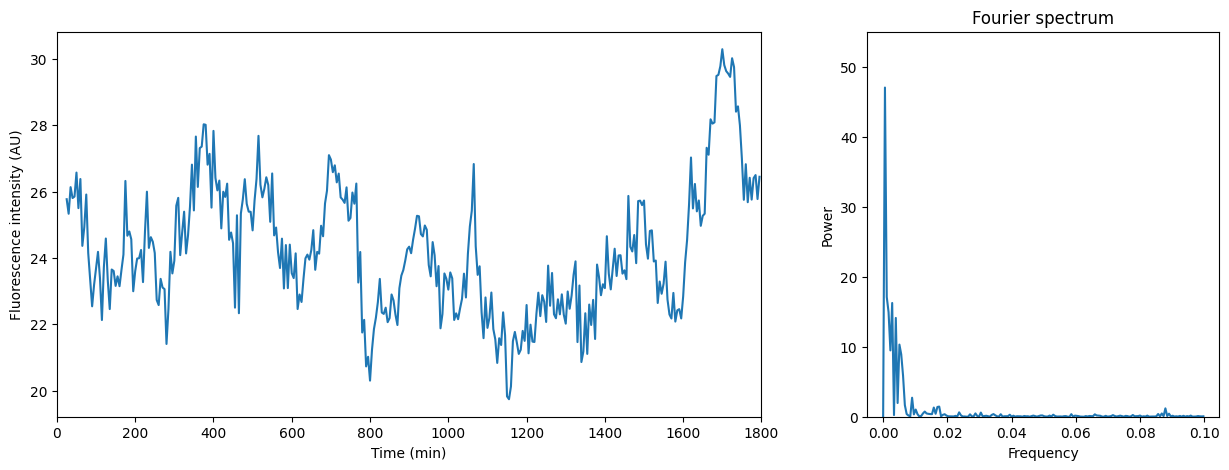
\includegraphics[width=\textwidth]{fft_raw}
   \caption{
   }
   \label{fig:analysis-filter-raw}
  \end{subfigure}

  \begin{subfigure}[htpb]{0.8\textwidth}
   \centering
   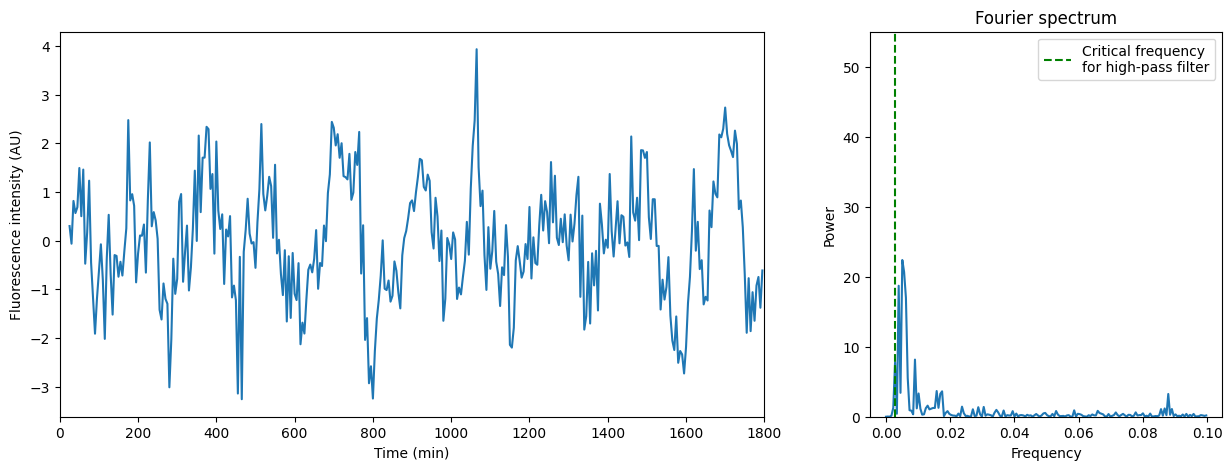
\includegraphics[width=\textwidth]{fft_butterworth}
   \caption{
   }
   \label{fig:analysis-filter-butterworth}
  \end{subfigure}

  \caption{
    (Left panels) Time series and (right panels) Fourier spectra corresponding to
    \textbf{(\ref{fig:analysis-filter-raw})}
    a sample raw time series of flavin autofluorescence, and
    \textbf{(\ref{fig:analysis-filter-butterworth})}
    the time series processed by a high-pass Butterworth filter with a critical frequency \SI[parse-numbers=false]{1/350}{\minute^{-1}}.
  }
  \label{fig:analysis-filter}
\end{figure}

To demonstrate the use of a method that modifies the frequency profile of time series to remove trends, Fig.\ \ref{fig:analysis-filter} shows how a time series and its Fourier spectrum changes after the application of a high-pass Butterworth filter with a critical frequency of \SI[parse-numbers=false]{1/350}{\minute^{-1}}.
Unlike sliding-window methods, defining a signal filter offers direct control over frequencies.
The critical frequency in this case was defined to create a reasonable upper limit of periods of the yeast metabolic cycle, based on my observations in single-cell microfluidics experiments.
Defining this critical frequency is a trade-off between emphasising metabolic oscillations in expected frequency windows and excluding the possibility of long-period metabolic cycles.


\begin{figure}
  \centering
  \begin{subfigure}[htpb]{0.8\textwidth}
   \centering
   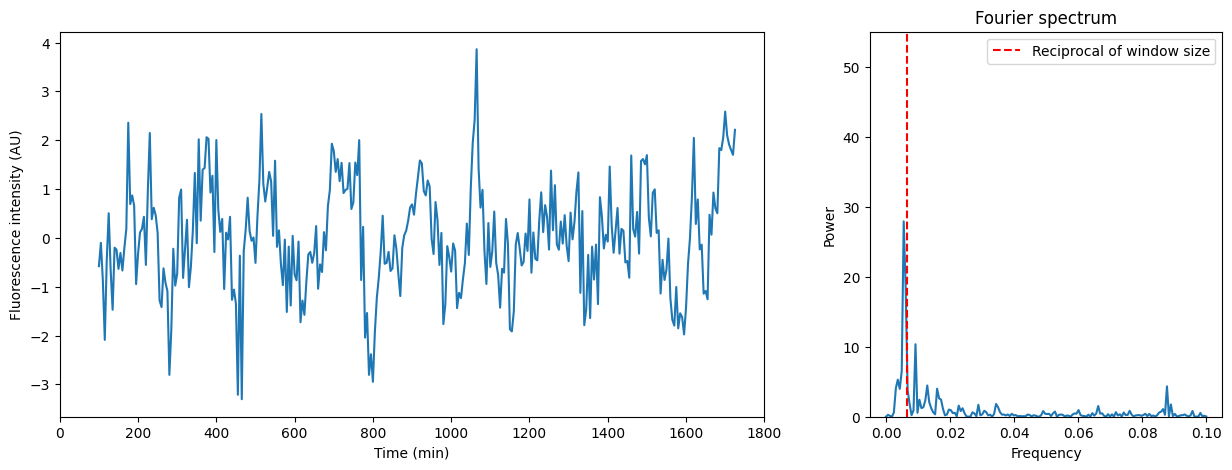
\includegraphics[width=\textwidth]{fft_slidingwindow}
   \caption{
   }
   \label{fig:analysis-slidingwindow-movavg}
  \end{subfigure}

  \begin{subfigure}[htpb]{0.8\textwidth}
   \centering
   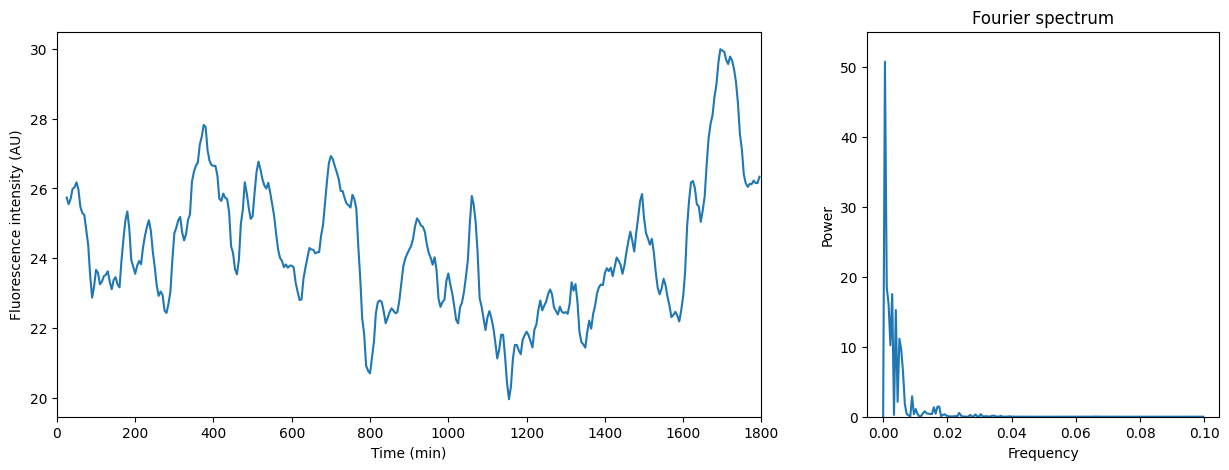
\includegraphics[width=\textwidth]{fft_savgol}
   \caption{
   }
   \label{fig:analysis-slidingwindow-savgol}
  \end{subfigure}

  \caption{
    (Left panels) Raw time series with trends, (middle panels) processed time series, and (right panels) Fourier spectra to demonstrate
    \textbf{(\ref{fig:analysis-slidingwindow-movavg})}
    using a moving average (window size 30), and
    \textbf{(\ref{fig:analysis-slidingwindow-savgol})}
    using a Savitzky-Golay filter (window size 7, polynomial order 3)
    to remove trends.
  }
  \label{fig:analysis-slidingwindow}
\end{figure}

To show how sliding-window methods adversely affect the frequency profile of time series when used for detrending, I computed the Fourier spectrum of time series detrended using the moving average method and the Savitzky-Golay filter.
Sliding-window methods are common in detrending biological time series.
For example, \textcite{cunyHighresolutionMassMeasurements2022} used a moving average: a constant, defined sliding window to smooth time series of yeast cell mass during growth.
\textcite{papagiannakisAutonomousMetabolicOscillations2017} fitted a smoothing spline to their single-cell fluorescence data of the yeast metabolic cycle, then divided the data points by the smoothing spline to detrend their data; the specific mathematical method used to define the smoothing spline was unclear in their study.
% Equations?
The Savitzky-Golay filter is also common --- this method is based on fitting a sliding window of a defined number of time points with a polynomial of a defined order using least squares fitting.

Fig.\ \ref{fig:analysis-slidingwindow-movavg} shows that the moving average method introduced an artefact in the frequency spectrum near the reciprocal of the window size and decreases the number of time points.
In contrast, Fig.\ \ref{fig:analysis-slidingwindow-savgol} shows that the Savitzky-Golay filter ...(INSERT DISCUSSION HERE)...
In sum, sliding-window methods were not ideal because they distorted the data in a way that affects conclusions, or removed noise information that may be useful.
% Really?
Importantly, it is not possible to restore the raw data when it is processed using such methods.

Therefore, for subsequent analyses, I used the high-pass Butterworth filter defined above to process raw fluorescence time series.
This is because using this method, I obtain more control over the frequency components, and the methods preserves noise frequencies that are useful for assessing the quality of the data set and estimating the noise properties.


\section[Classification]{Classification: is my time series oscillatory?}
\label{sec:analysis-classification}

To assess how a perturbation affects the YMC, it is important to have a systematic method to determine whether a time series is oscillatory.
% However, there are challenges with classification of noisy biological time series with relatively few time points.
% In addition, such a classification task necessarily needs a cut-off somewhere, thus requiring judgement calls.
% You'd see this crop up in this section multiple times when I discuss my methods and I reveal different angles of approaching this.
Determining whether a time series is oscillatory, or rhythmicity detection, is technically difficult for several reasons.
From a signal processing perspective, any time-dependent signal can be decomposed into a combination of sinusoids of different frequencies.
Noise typically manifests as high-frequency components while trends manifests as low-frequency components --- the filtering methods in section~\ref{sec:analysis-cleaning} arise because of this fact.
It is thus more reasonable to detect the presence of a frequency within the range of interest.
However, this depends on knowing an expected range of frequencies.
When studying the circadian rhythm, this is often the case: studies expect rhythms of around \SI{24}{\hour} and \textcite{zielinskiStrengthsLimitationsPeriod2014} uses the range of \SIrange{16}{32}{\hour} for rhythmicity detection.
This method is less useful when the frequency of oscillations is unknown or known to be in a wide range of frequencies, as is the case for the yeast metabolic cycle.
Furthermore, there is no way to objectively specify a failure rate for a rhythmicity detection method as there is no independent method to estimate rhythmicity \parencite{zielinskiStrengthsLimitationsPeriod2014}, therefore such a classification method requires a subjective definition of whether each time series is oscillatory.
In other words, this is similar to the requirement of a training data set with human-defined labels, and thus a human-defined failure rate, for supervised machine learning.

In this section, I will discuss my use of spectral methods, model-fitting methods, and machine learning methods.

% Literature review subsection

% - Compare and contrast methods
% - Highlight challenges with large datasets of noisy biological data
% - Review existing methods first and then talk about the methods I tried, with results.
%   FFT (already copied from 10m, to be re-written slightly), AR (steal figures from AC22 poster & presentations made in that time)

\subsection{Rhythmicity detection using spectral methods}
\label{subsec:analysis-classification-spectral}

% Copied from 10m report
% ----------------------
% Minireview of studies about finding whether there is an oscillation in circadian time series (or other related time series) -- keep it relatively short.

% Discussion about oscillatory behaviour vs periodic behaviour?

\textcite{glynnDetectingPeriodicPatterns2006} describe a method to classify gene expression profiles as oscillating or non-oscillating based on the Lomb-Scargle periodogram \parencite{lombLeastsquaresFrequencyAnalysis1976}.
This periodogram was developed for time series with missing time points, and has a chi-square distribution that aids a statistical test for periodicity \parencite{scargleStudiesAstronomicalTime1982}.
The classification was based on controlling the false discovery rate for identification of oscillations.
In testing multiple hypotheses, the false discovery rate is defined as the proportion of cases in which the null hypothesis is true among all hypotheses in which the test is declared significant.
Increasing the false discovery rate thus increases the proportion of time series classed as oscillating.

I developed a classifier based on \textcite{glynnDetectingPeriodicPatterns2006} to classify time series of flavin autofluorescence as follows:

\begin{enumerate}
\item Let the data have $\mathcal{G}$ cells.
Let cell $g = 1, \dots{}, \mathcal{G}$ have a time series with $N_{g}$ time points.
The time series is thus denoted $Y_{g}(t) = y_{g}(t_{1}), \dots{}, y_{g}(t_{N_{g}})$.
\item For each time series, I define a range of test frequencies linearly from $\frac{1}{N_{g}}$ to the Nyquist limit (i.e. half the rate of image acquisition, \SI{0.2}{\minute^{-1}}, in this case).

With this definition, I compute the classical periodogram for each time series:
  \begin{equation}
    P_{g}(\omega) = \frac{N_{g}}{2\sigma^{2}} \left|\int_{-\infty}^{\infty} Y_{g} e^{-2\pi it}dt \right|, % check constants, etc
    \label{eq:normalised-periodogram}
  \end{equation}
        where $\sigma^{2}$ is the sample variance of $Y_{g}$.
        In this equation, the periodogram is normalised by the coefficient $N_{g}/2\sigma^{2}$ so that the area under the periodogram is constant across all time series.
        The Lomb-Scargle periodogram is equivalent to the classical periodogram if the time points are equally spaced \parencite{lombLeastsquaresFrequencyAnalysis1976}, as is the case for the vast majority of my data.
\item For each cell $g$, I denote the peak $h_{g} = \max_{j}P_{g}(\omega)$.
I define an effective number of independent frequencies $M = f_{max}N_{g}$ for each time series, where $f_{max}$ is the Nyquist limit \parencite{vanderplasUnderstandingLombScarglePeriodogram2018}.
  I then calculate the $p$-value of testing the null hypothesis that such a peak is due to chance:
  \begin{equation}
    p_{g} = 1 - (1 - e^{-h_{g}})^M
    \label{eq:lsp-pval}
  \end{equation}
  This formula is based on the exponential distribution of the power at a given frequency in the periodogram \parencite{scargleStudiesAstronomicalTime1982}.
\item I order the cells by $p$-values: $p_{(1)} \leq p_{(2)} \leq \dots \leq p_{(\mathcal{G})}$.
  To control the false discovery rate \parencite{benjaminiControllingFalseDiscovery1995}, I find $\hat{k}$ according to:
  \begin{equation}
    \hat{k} = \arg\max_{1 \leq k \leq \mathcal{G}}\{k : p_{(k)} \leq qk/\mathcal{G}\}
    \label{eq:lsp-khat}
  \end{equation}
  where $q$ is a defined false discovery rate.
\item Cells whose $p$-values correspond to $p_{(1)}, p_{(2)}, \dots, p_{(\hat{k})}$ are thus denoted to have statistically significant oscillatory behaviour for the false discovery rate $q$.
\end{enumerate}

%I then compared the classification results against manual classification of these time series into oscillating and non-oscillating.
The classifier was able to rank the time series by quality of oscillation (figure \ref{fig:ClassifierBestWorstTS}).
The peak of the normalised classical periodogram of each time series was used as a proxy for the quality of oscillation (figure \ref{fig:ClassifierBestWorstPS}).
By eye, birth events coincided with peaks of some higher-quality oscillations.
However, this was also true for some oscillations ranked as lower-quality.
% [COMMENTED -- don't think this sentence is really consequential, and the proposed plot doesn't add much] Additionally, higher-quality oscillations do not seem to be associated with imaging positions/flavin LED exposure times. % FIGURE: scatter plot, horizontal axis is rank, vertical axis is imaging position
% Wee bit of discussion (plus a plot to illustrate my point).  Deeper discussion about multiple main frequencies is in discussion, and has references to literature.
These oscillations were ranked as low-quality because the Fourier transform identified multiple main frequencies, and thus lowered the peak of the normalised periodogram.
Thus, a Fourier-based method may not adequately provide the information for a reliable ranking of oscillation quality.

\begin{figure}[htbp]
  \centering
  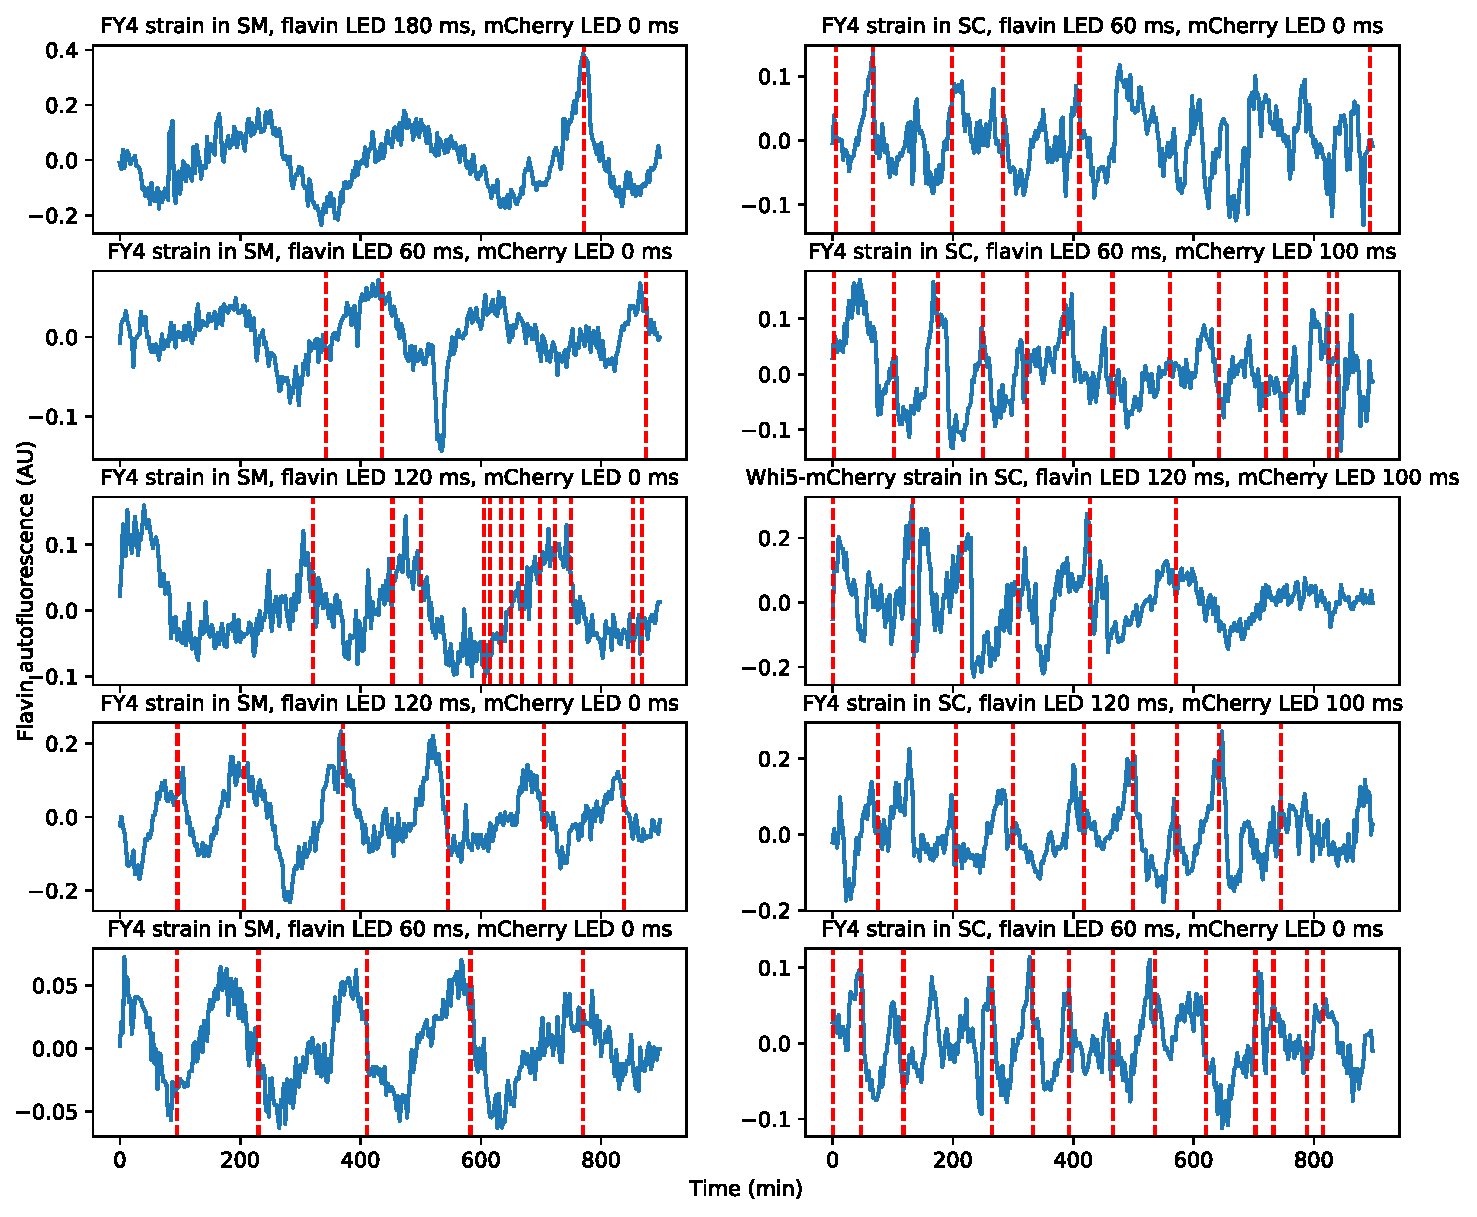
\includegraphics[width=\textwidth]{10m_ClassifierBestWorstTS}
  \caption[
    Classifier based on Lomb-Scargle periodogram ranks time series by quality of oscillation
  ]{
    Classifier based on Lomb-Scargle periodogram ranks time series by quality of oscillation.
    Left column shows `best' five and right column shows `worst' five.
    Blue solid lines: flavin autofluorescence, red dashes: birth event automatically identified by \textit{BABY}.
  }
  \label{fig:ClassifierBestWorstTS}
\end{figure}

\begin{figure}[htbp]
  \centering
  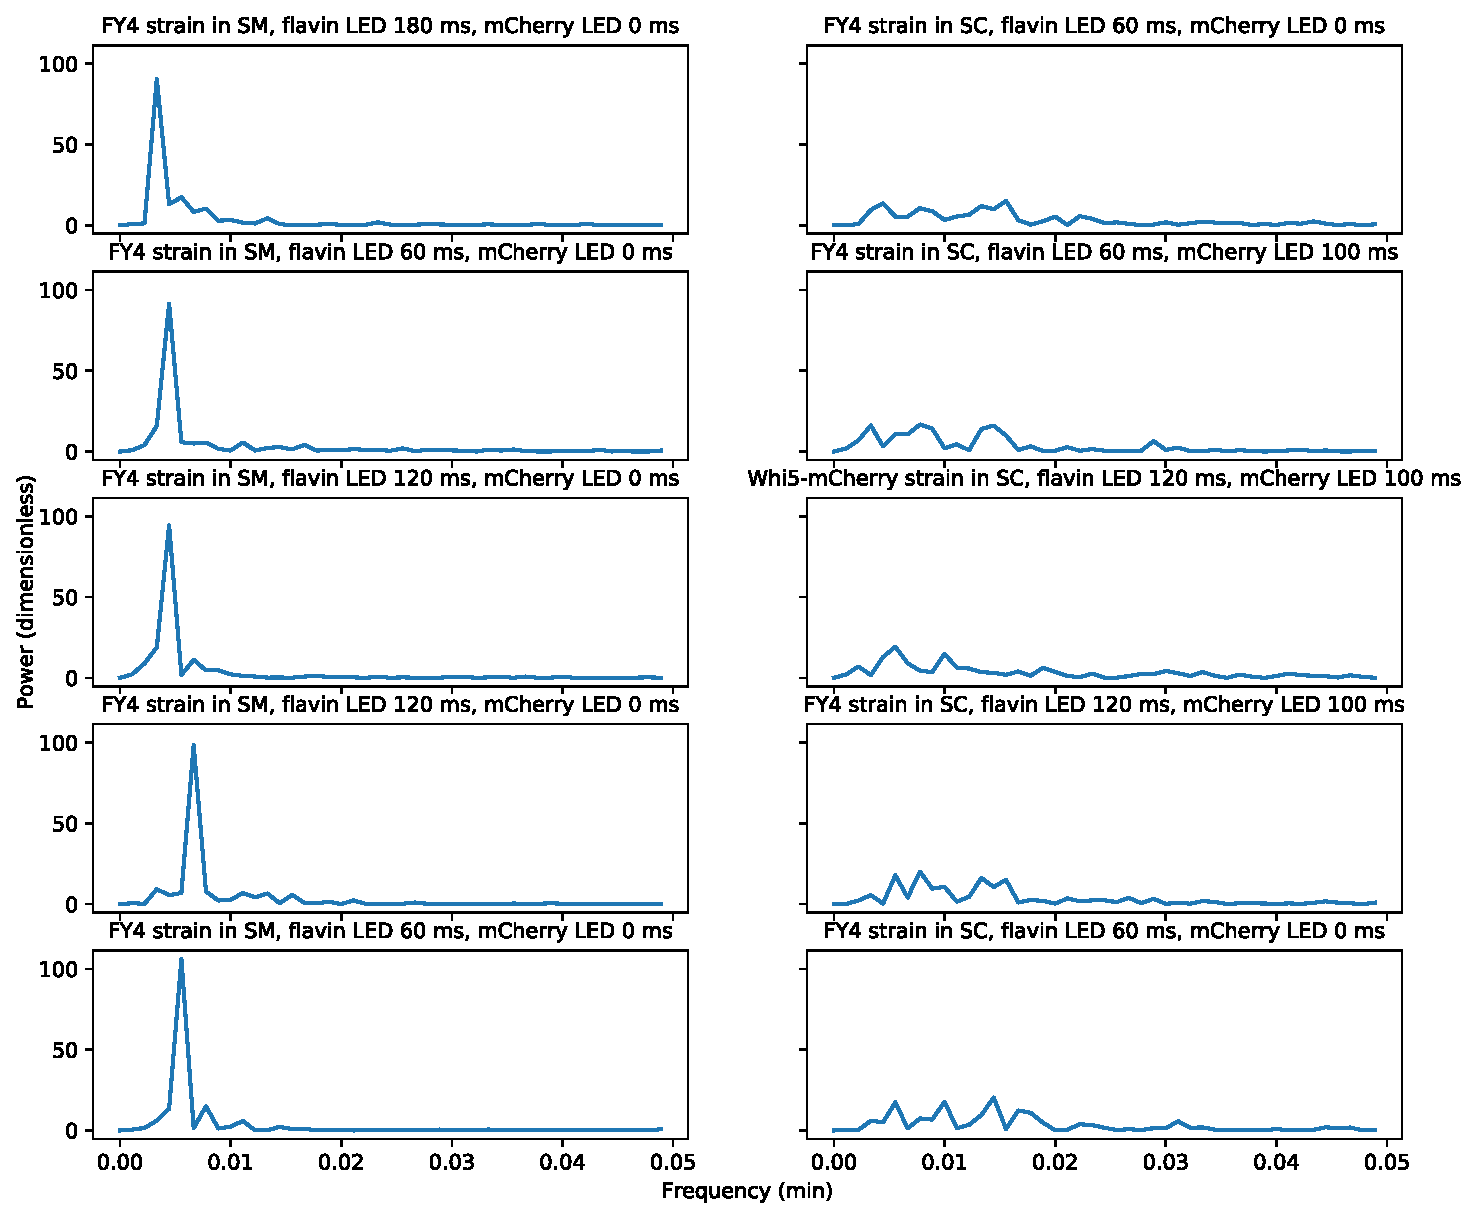
\includegraphics[width=\textwidth]{10m_ClassifierBestWorstPS}
  \caption[
    Highest peak of normalised classical periodograms is an inadequate proxy for quality of oscillations
  ]{
    Highest peak of normalised classical periodograms is an inadequate proxy for quality of oscillations.
    Blue solid lines: normalised classical periodograms of time series in figure \ref{fig:ClassifierBestWorstTS}.
  }
  \label{fig:ClassifierBestWorstPS}
\end{figure}

The classifier has multiple caveats.
It one tuning parameter, the false discovery rate, and its value affects the proportion of time series classed as oscillating.
I resorted to subjective judgements of whether a time series exhibited oscillations, and thus any optimised false discovery rate would have low reliability.
A reliable ground truth is needed to optimise the value of the false discovery rate so that the classification accuracy is maximised.
Such a ground truth would ideally be from an experiment that is expected to give rise to time series that are not oscillatory.

\subsection{Rhythmicity detection using model fitting}
\label{subsec:analysis-classification-ar}

The autoregressive model has been used before to characterise biological time series \parencite{zielinskiStrengthsLimitationsPeriod2014}.
This model is based on the assumption that each data point in the time series can be expressed as a linear combination of $P$ data points that precede it --- $P$ thus representing the order of the model.
This autoregressive model thus `smooths' the time series.

\textcite{jiaFrequencyDomainAnalysis2021} describe an application of the autoregressive model, based on the fact that there is an analytical solution for the periodogram based on this model.
This publication describes a model of stochastic gene expression in a dividing cell, which predicts oscillatory gene expression.
Autoregressive models were fitted to simulated time series of oscillatory gene expression, and its parameters used to define a power spectrum for the time series.
I implemented this algorithm, described by \textcite{jiaFrequencyDomainAnalysis2020}, as follows:

\begin{enumerate}
  \item The algorithm relies on fitting a single time series $n(0), n(1), \ldots , n(M-1)$ with an autoregressive model $\mathrm{AR}(P)$ with order $P$:
        \begin{equation}
          \label{eq:ar-model}
          \phi_{0}n_{t} + \phi_{1}n_{t-1} + \phi_{2}n_{t-2} + \ldots + \phi_{P}n_{t-P} = \theta_{0}\epsilon_{t}
        \end{equation}
        where $\epsilon_{t}$ is a white noise satisfying $\langle \epsilon_{t} \rangle = 0$,
        $\phi_{0} = 1$, and
        $\phi_{1}, \ldots , \phi_{P}$ are real numbers such that the complex zeros of the polynomial $\Phi (z) = \sum_{k=0}^{P} \phi_{k}z^{k}$ lie outside the unit circle.
  \item The sample mean of the time series is estimated by:
        \begin{equation}
          \label{eq:ar-mean}
          \langle n \rangle = \frac{1}{M} \sum_{k=0}^{M-1}n(k)
        \end{equation}
  \item The sample autocorrelation function is estimated as:
        \begin{equation}
          \label{eq:ar-acf}
          R_{i} = \frac{1}{M} \sum_{k=0}^{M-1-i}(n(k) - \langle n \rangle)(n(k+i) - \langle n \rangle)
        \end{equation}
  \item The coefficients $\phi_{1}, \ldots , \phi_{P}$ are estimated by solving the Yule-Walker equation:
        \begin{equation}
          \label{eq:ar-yule-walker}
          \begin{bmatrix}
            R_{0} & R_{1} & \dots & R_{P-1} \\
            R_{1} & R_{0} & \dots & R_{P-2} \\
            \vdots & \vdots & \ddots & \vdots \\
            R_{P-1} & R_{P-2} & \dots & R_{0}
          \end{bmatrix}
          \begin{bmatrix}
            \phi_{1} \\
            \phi_{2} \\
            \vdots \\
            \phi_{P}
          \end{bmatrix}
          =
          \begin{bmatrix}
            R_{1} \\
            R_{2} \\
            \vdots \\
            R_{P}
          \end{bmatrix}
        \end{equation}
  \item The parameter $\theta_{0}$ is estimated as:
        \begin{equation}
          \label{eq:ar-noise-param}
          \theta_{0}^{2} = R_{0} - \sum_{k=1}^{P}\theta_{k}R_{k}
        \end{equation}
  \item The order $P$ is determined by minimising the Akaike information criterion:
        \begin{equation}
          \label{eq:ar-aic}
          \mathrm{AIC}(P) = \log \theta_{0}^{2}(P) + 2 \frac{P}{M}
        \end{equation}
        where $\theta_{0}(P)$ is the estimated $\theta_{0}$ (equation~\ref{eq:ar-noise-param}) for a specific $P$.
        In this step, $P$ is varied with $1 \leq P \leq 3 \sqrt{M}$, and the optimum order ($P$) is the one that gives the smallest value of $\mathrm{AIC}(P)$
   \item The power spectrum is thus estimated analytically using the parameters found in earlier steps by:
        \begin{equation}
          \label{eq:ar-power-spectrum}
          G(\xi) = \frac{1}{2 \pi} \cdot \frac{\theta_{0}^{2}}{|\sum_{k=0}^{P}\phi_{k}\me^{-ik\xi}|^{2}}, -\pi \leq \xi \leq \pi
        \end{equation}
        where $\xi$ represents frequency.
\end{enumerate}

\begin{figure}
  \centering
  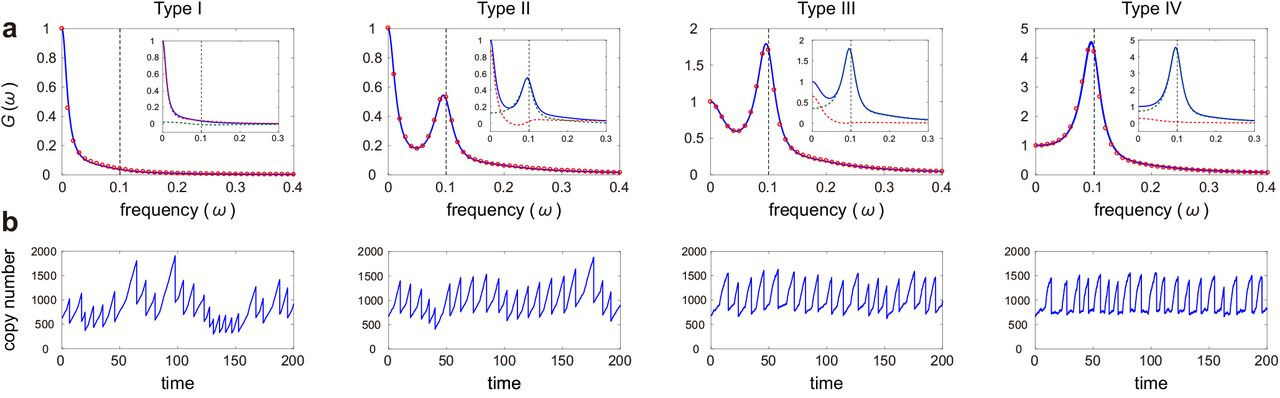
\includegraphics[width=0.9\textwidth]{jiaFrequencyDomainAnalysis2020_2ab_adapted}
  \caption[
    Power spectra analytically derived from fitting an autoregressive model to time series can be divided into four types
  ]{
    Power spectra (a) analytically derived from fitting an autoregressive model to time series (b) can be divided into four types.
    Type I lacks a local maximum and is denoted as lacking oscillations.
    Figure adapted from \textcite{jiaFrequencyDomainAnalysis2020}.
  }
  \label{fig:analysis-ar-classification}
\end{figure}

The resulting power spectra fell into four categories: one of which corresponded to a lack of oscillations, characterised by an absence of a local maximum in the power spectrum (figure~\ref{fig:analysis-ar-classification}).
This method thus makes it easy to compute the frequency of the oscillation from the location of the peak and quality of the oscillation from the height of the peak, as opposed to a Fourier spectrum computed base on noisy data.

\begin{figure}
  \centering
  \begin{subfigure}[htpb]{0.6\textwidth}
   \centering
   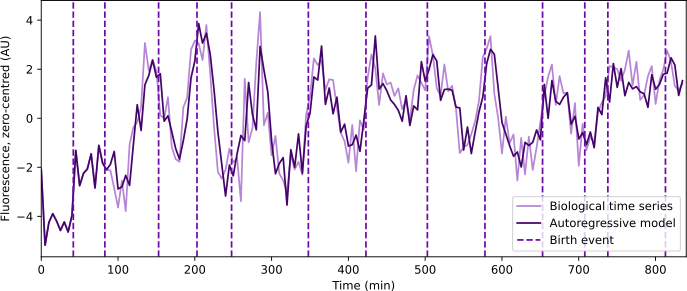
\includegraphics[width=\textwidth]{timeseries_example_for_ar}
   \caption{
     Example time series to illustrate the autoregressive model fitting method.
     The original time series is shown in light purple, and the autoregressive model with order 4 is fitted to produce the time series shown in dark purple.
     Birth events automatically defined by \textit{BABY} are shown in dashed vertical lines.
   }
   \label{fig:analysis-ar-timeseries}
  \end{subfigure}%
  \begin{subfigure}[htpb]{0.4\textwidth}
   \centering
   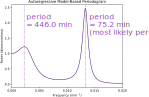
\includegraphics[width=\textwidth]{ar}
   \caption{
     The fitted model in~\ref{fig:analysis-ar-timeseries} leads to an analytical definition of a periodogram.
     The presence of peaks indicate that the time series is oscillatory.
     In this case, the peaks in the periodogram gives a good estimate of the most likely period of oscillation in the original time series.
   }
   \label{fig:analysis-ar-periodogram}
  \end{subfigure}
  \caption{
    Fitting an autoregressive model to determine period.
  }
  \label{fig:analysis-ar}
\end{figure}

Figure~\ref{fig:analysis-ar} shows an example of the autoregressive model method performed on my time series data of flavin autofluorescence.
In my investigations, very few time series within a dataset were classified as oscillatory using this method.
The problem is that there are no parameters that I can adjust to change the `tolerance' for detecting rhythmicity.
However, among the time series that it deems oscillatory, it guesses the frequency fairly well.
%[Need: figures to summarise my investigation on population.  Probably need to re-do this on some datasets because it is poorly documented in my notes.]
Alternatively, I can treat the order of the model as a parameter, and perform model selection on it.

% This subsection needs better re-organisation.
% I've done some attempts by putting some headers in comments.
% But perhaps a better way is to draft some `summary' figures to show key takeaways, and then let the text flow accordingly.
\subsection{Machine learning approaches to classification}
\label{subsec:analysis-classification-ml}
% - Write results from classifier project (SVM, RF, etc.)

% Copied from org note: 'Using SVM with a population of cells', which isn't particularly well-written.
% ----------------------

% [TODO] Worth re-doing the whole experiment using better data, e.g. the data I'm actually using in the biological results chapter.

% OVERVIEW OF MACHINE LEARNING
% (needed to make the rest of the section make sense)
In machine learning, classification is defined as the process of identifying a category that a piece of input data belongs to.
In the context of this section, the classification task is identifying whether a time series (input data) is oscillatory (belongs to one category of two) or non-oscillatory (belongs to the other category of two).

When performing a classification task, input data is first converted to feature vectors in the process of featurisation.
This process uses domain knowledge related to the type or origin of the data to define characteristics of the data that may be useful for classification.
Each piece of input data has a label assigned to it to denote which category it belongs to.
The input data set is then divided into a training data set and a test data set.
The machine learning model is then fit on the training data set to fit parameters in the model, and then the performance of the model is evaluated on the test data set.
Such model evaluation is based on quantitative measures of how well the model matches data to appropriate labels.

% DESCRIPTION OF DATA

For this section, I used data from BY4741 cells under \SI{10}{\gram~\litre^{-1}} glucose, before any nutrient changes.
% -----[Probably no need to go into so much detail.]-----
% I removed the first 25 time points that is most likely cells adapting to microfluidic conditions.
% I also removed time points after time point 168, when nutrient switching occurred.
% I removed all time series with missing time points.
In total, there are 294 cells, each with 118 time points, spaced 5 minutes apart.

% DATA PROCESSING

% [TODO] Repeat experiment with Butterworth filter, rather than sliding window detrending

% Figure ... shows a clear downwards trend (which I can't explain biologically yet). If an SVM model is trained using time points as features, there is a risk that the model recognises this trend rather than the presence of oscillations.
% This plot highlights the risk: for some reason non-oscillating time series (hand-scored) tends to have a smaller gradient.
% I thus detrended the data by generating a moving average with a sliding window size of 45 time points, and then dividing each data point by the moving average. I chose 45 time points because that covers ~3 cell division cycles.
% However, there are caveats.
% If the cell division cycle length differs, this window length should change; a spectral method (FFT, autoregressive) could give me an idea of what this cell division cycle length is.
% Additionally, this decreases the number of time points --- there are now 98.

The dynamic range of each time series are different from each other, so I additionally normalised each time series $x_{i}$ by computing the standard score:

\begin{equation}
  \label{eq:analysis-stdscore}
  z_{i,j} = \frac{x_{i,j} - \mu_{i}}{\sigma_{i}}
\end{equation}

where $i$ represents each time series, $j$ represents each time point which a time series, $\mu_{i}$ is the mean value of each time series across its time points, and $\sigma_{i}$ is the standard deviation of the values within each time series across its time points.
As a result, each normalised time series has a mean of 0 and a standard deviation of 1.

% LABELLING

Based on the processed data, I manually scored the 294 time series as non-oscillatory (label `0') or oscillatory (label `1').
Here, there are 211 oscillatory time series (72\%) and 83 non-oscillatory time series (28\%).
Thus, there is a slight class imbalance.
% SPLITTING
I chose 150 time series at random to be used as training data --- the rest becomes testing data.
% FEATURISATION
And, I explored three methods of featurisation: using time points as features, the time series' Fourier spectrum as features, and using \textit{catch22} features \parencite{lubbaCatch22CAnonicalTimeseries2019}.

\textit{catch22} is based on the \textit{hctsa} toolbox \parencite{fulcherHctsaComputationalFramework2017} developed to compute vectors of features for time series.
This toolbox contains 7701 features defined from across the time series analysis literature.
I focused on the 22-feature \textit{catch22} subset of the original 7701 features (table \ref{tab:catch22}).
\textcite{lubbaCatch22CAnonicalTimeseries2019} selected these 22 features because they minimise redundancy while maintaining classification performance across 93 test datasets.
This feature set excludes features that are dependent on mean or spread.

After featurisation, to account for the different dynamic ranges of each feature, the features were scaled by computing the standard score, similar to equation~\ref{eq:analysis-stdscore}.

% MODELS

I explored support vector machine (SVM) and random forest (RF) model architectures.
First, I used an support vector classifier (SVC) with these hyperparameters:
\begin{enumerate}
  \item A radial bias kernel.
  \item The kernel coefficient $\gamma = 1/N$, where $N$ is the number of features.
  \item The regularisation parameter $C = 1$.  The strength of regularisation is inversely proportional to $C$.
\end{enumerate}

\begin{figure}
  \centering
  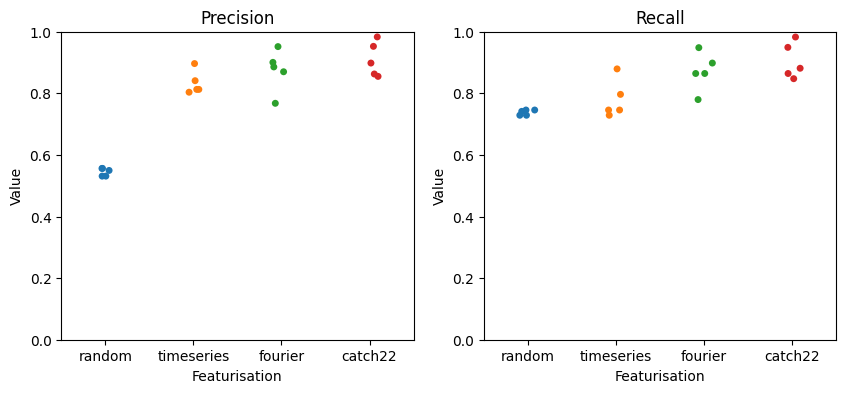
\includegraphics[width=0.9\textwidth]{precision_recall}
  \caption[
    Featurisation strategies for a support vector classifier to classify oscillatory time series of flavin autofluorescence
  ]{
    Evaluation of featurisation strategies for a support vector classifier to classify oscillatory time series of flavin autofluorescence.
    Precision and recall were used as evaluation metrics, and data points represent each of the five rounds of five-fold cross-validation.
  }
  \label{fig:analysis-precision-recall}
\end{figure}

As a control, I randomly assigned time series to the oscillatory and non-oscillatory categories and used their time series as features.
I then evaluated the model using stratified five-fold cross-validation, using precision and recall as evaluation metrics.
Using time points as features, the metrics show that precision and recall is better than random, and stratified five-fold cross-validation does not suggest overfitting (figure~\ref{fig:analysis-precision-recall}).
Using the Fourier spectrum as features, precision and recall are comparative as with using time points as
features.
However, there seems to be greater variation in these measures.


\begin{figure}
  \centering
  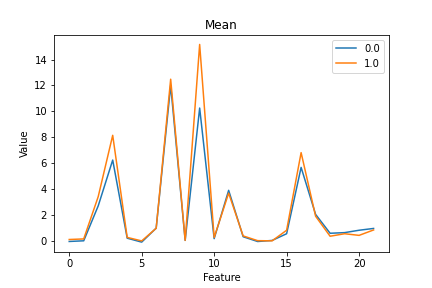
\includegraphics[width=0.5\textwidth]{catch22_training_featurevector_mean}
  \caption[
    Mean values of each \texttt{catch22} feature across each cell
  ]{
    Mean values of each \texttt{catch22} feature across each cell classified as non-oscillatory (class 0) or oscillatory (class 1) by an SVC from the testing set.
    The horizontal axis shows each \texttt{catch22} feature from 0 to 21, and the vertical axis shows the mean value of each feature across cells within an identified class.
  }
  \label{fig:analysis-svc-catch22}
\end{figure}

Nevertheless, precision and recall are best with \textit{catch22}.
Feature vectors seem to suggest that the \texttt{FC\_LocalSimple\_mean3\_stderr} feature (represented as feature 9 in figure~\ref{fig:analysis-svc-catch22}) plays an important role in distinguishing the oscillatory and non-oscillatory time series.
This feature is defined as the mean error from a rolling 3-sample mean forecasting.

%[CONFIRM IMPORTANCE VIA RECURSIVE FEATURE ELIMINATION, USING RANDOM FOREST?]

% ADAPTATION OF SVM: PREDICT PROBABILITIES

% Include result from randomly assigning labels as a control?
% This should give a `hill' in the middle.
\begin{figure}
  \centering
  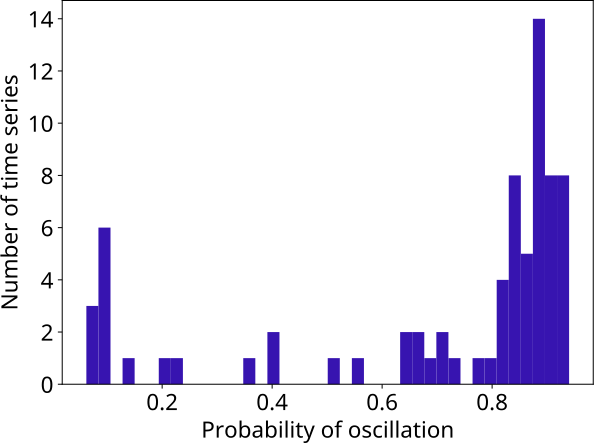
\includegraphics[width=0.5\textwidth]{classifier_histogram_probabilities_adapted}
  \caption{
    Histogram of probabilities of whether a time series in the test data set is classified as oscillatory by the SVC.
  }
  \label{fig:analysis-svc-proba-histogram}
\end{figure}


\begin{figure}
  \centering
  \begin{subfigure}[t]{0.45\textwidth}
  \centering
    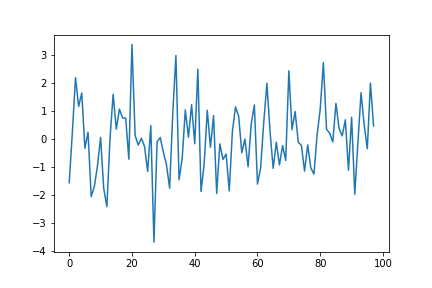
\includegraphics[width=\linewidth]{proba_00}
    \caption{
      0\%
    }
    \label{fig:analysis-svc-proba-00}
  \end{subfigure}%
  \begin{subfigure}[t]{0.45\textwidth}
  \centering
    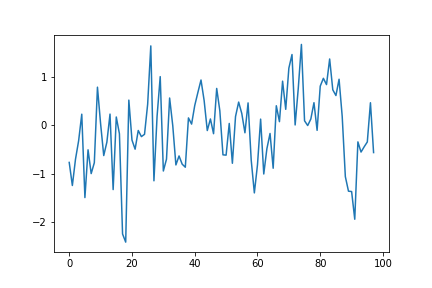
\includegraphics[width=\linewidth]{proba_21}
    \caption{
      21\%
    }
    \label{fig:analysis-svc-proba-21}
  \end{subfigure}

  \begin{subfigure}[t]{0.45\textwidth}
  \centering
    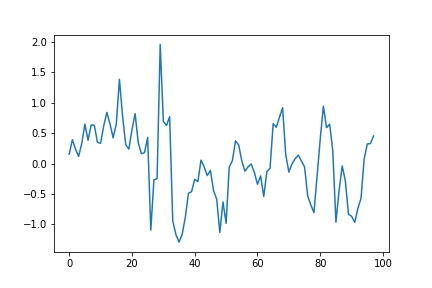
\includegraphics[width=\linewidth]{proba_38}
    \caption{
      38\%
    }
    \label{fig:analysis-svc-proba-38}
  \end{subfigure}%
  \begin{subfigure}[t]{0.45\textwidth}
  \centering
    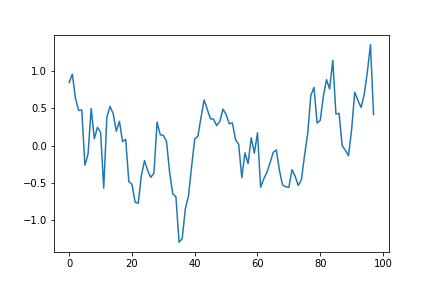
\includegraphics[width=\linewidth]{proba_61}
    \caption{
      61\%
    }
    \label{fig:analysis-svc-proba-61}
  \end{subfigure}

  \begin{subfigure}[t]{0.45\textwidth}
  \centering
    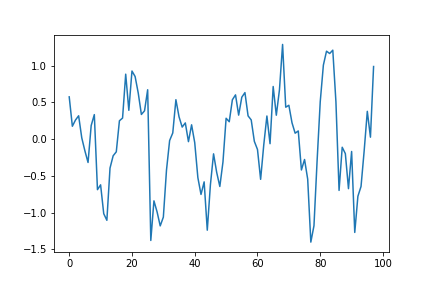
\includegraphics[width=\linewidth]{proba_88}
    \caption{
      88\%
    }
    \label{fig:analysis-svc-proba-88}
  \end{subfigure}%
  \begin{subfigure}[t]{0.45\textwidth}
  \centering
    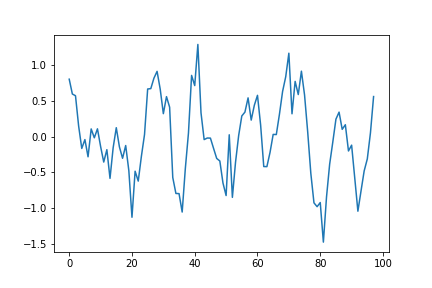
\includegraphics[width=\linewidth]{proba_99}
    \caption{
      99\%
    }
    \label{fig:analysis-svc-proba-99}
  \end{subfigure}
  \caption{
    Test set time series shown by probability that each is oscillatory, as determined by the SVC.
  }
  \label{fig:analysis-svc-proba-gallery}
\end{figure}

Using the \textit{catch22} features, I extended the support vector classifier enabling probability estimates, so that the model computes the probability that a time series is oscillatory, rather than assign one of two outputs.
Figure~\ref{fig:analysis-svc-proba-histogram} show that the distribution of probabilities falls in a U-shape; this distribution is desirable because it means that the classifier is for the most part `certain' whether a time series is oscillatory or not.
In addition, these probabilities can also serve as a score for the quality of oscillations, as illustrated by figure~\ref{fig:analysis-svc-proba-gallery}.

%[MORE EVALUATION? e.g. ROC curve, precision-recall curve.  MAYBE IT IS OVERKILL HERE.]

In sum,
% I mention modularity clustering before its appropriate section here.
% I can create a reference to that section, or move this paragraph to that section and re-word it a bit so it fits the logical flow.
% ------------------------------------
the \textit{catch22} features seem to function best.
%It makes sense -- given that I could plot cells in \texttt{catch22} feature space and perform modularity clustering, an SVM model based on drawing a `lane' between two clouds of points in \texttt{catch22} feature space should work.
%Furthermore,
%\textcite{lubbaCatch22CAnonicalTimeseries2019} has tested the features' ability to categorise time series across multiple large datasets.
A simple machine learning architecture is sufficient in classifying noisy biological time series into oscillatory and non-oscillatory categories, complete with probabilities.
This method was also able to identify which time series feature was the most important in distinguishing between oscillatory and non-oscillatory time series.

\section[Characterisation]{Characterisation: I have one time series --- what properties does it have?}
\label{sec:analysis-characterisation}

The importance of characterising my time series is that I can quantify how my yeast metabolic cycles respond to genetic and nutrient perturbations.
Here, I discuss characterising periods, phases, and amplitudes of the oscillations.
%Note that I discuss many of the same non-machine learning methods as I did for the classification section -- such methods are often developed for characterisation but offer features that are useful for classification, but it makes more sense in my thesis to order it this way because you'd usually try to filter out the non-oscillatory time series before trying to grab properties of the oscillatory ones.
Then I will discuss the merit of combining several methods, given the limitations of analysing noisy biological time series that I have found.
% [THIS SENTENCE MAY GO]
%Characterisation is also intimately related to classification, in particular the machine learning methods: these methods can be adapted to tell apart different strains (presumably of different shapes) rather than telling apart oscillatory and non-oscillatory time series.

% Literature review subsection
% STEAL IDEAS FROM: ZIELINSKI ET AL. 2014
\subsection{Periods, phases, amplitudes}
\label{subsec:analysis-characterisation-quantities}

Three useful characteristics of a time series include its period, its phase relative to a reference, and its amplitude.
% Adapted from meeting with Zielinski.
% TODO with this:
% - support with evidence, e.g. discussion points from his paper and others

% PERIOD
The period of an oscillatory time series is the easiest characteristic to compute a fixed number for because it is well-defined.

% SHAPE
The shape of oscillations in a time series is difficult to analyse and assign a meaningful quantitative measure to --- it is easier to describe the shape by eye.
From the signal processing point of view, the shape of an oscillation is defined by a set of frequencies of sinusoids and their respective power values.
In other words, to quantitatively describe the shape of an oscillation, a vector of values is needed, and any fixed-number representation necessarily removes some information about the shape.
Alternatively, the shape can be expressed in terms of skewness, treating one oscillation as if it were a probability distribution. %[CITATION NEEDED].

% PHASE
There are challenges in obtaining a fixed number of represent the phase of an oscillator time series based on the signal.
Most importantly, the phase must be defined with respect to a human-defined reference, which may not be clear depending on the data.
In addition, the phase angle can have uncertainty, particularly if the time series is noisy.
Phase estimation is part of period estimation methods that are based on fitting cosines to data (to be discussed later), and an error range will always be given.
Estimating the phase angle also requires multiple replicates as estimation methods rely on plotting populations of time series and seeing if they overlap.
Modular arithmetic is also needed for such methods.
In sum, more information is needed to estimate the phase compared to other methods.
When a quantitative representation of the phase is obtained, it can be expressed in absolute terms (in units of time), or in relative terms with respect of the period (in radians).

% AMPLITUDE
The amplitude of the time series is easiest to compute and easiest to explain.
Methods to estimate the amplitude relies on fitting a cosine to the signal.
Such methods are adequate if the shape of the time series does not change by much across time, but are inadequate if oscillations are skewed, as the cosine function models symmetrical oscillations.
However, the amplitude is likely the least important characteristic to study in the biological timekeeping field.

Of these, finding the period is the easiest to do and most pertinent for my investigation of the yeast metabolic cycle, so I focus my further discussion on period estimation.
Another common period-estimation method relies on the autocorrelation function, and it was used in \textcite{papagiannakisAutonomousMetabolicOscillations2017}.
Here, I am going to discuss adapting the autocorrelation function for my data.

\subsection{Autocorrelation function}
\label{subsec:analysis-characterisation-acf}

In this section, I show that the autocorrelation function can be adapted to characterise the period and noise properties of populations of both sinusoid time series and time series and asymmetrical oscillations.
I first do so with synthetic time series with known properties and adapt the methods to my data that exhibit similar oscillations as the synthetic time series.

\subsubsection{Mathematical definitions}
\label{subsubsec:analysis-characterisation-acf-maths}

The cross-correlation function used in this chapter is adapted from \textcite{pietschDeterminingGrowthRates2023}, as follows:

\begin{enumerate}
  \item Let the data have $M$ cells.
        Each cell $i$ in the population of $M$ cells has a time series $x_{1}^{(i)}, \ldots , x_{j}^{(i)}, \ldots , x_{N}^{(i)}$ of quantity $x$ and a time series $y_{1}^{(i)}, \ldots , y_{j}^{(i)}, \ldots , y_{N}^{(i)}$ of quantity $y$.
        Let both time series have a sampling interval of $\Delta t$.
  \item The deviation from the population mean for each time series is computed.
        This population mean is calculated over replicates at each time point.
        The caveat of this calculation is that the signals \emph{must} be out-of-phase, and I ensure this by generating synthetic signals with a random phase.
        Otherwise, the underlying signal will be subtracted from all time series and the cross-correlation of noise will be computed --- this is undesired.
        \begin{equation}
          \delta x_{t}^{(i)} = x_{t}^{(i)} - \frac{1}{M} \sum_{j}x_{t}^{(j)}
          \label{eq:xcf-dmeans-x}
        \end{equation}
        \begin{equation}
          \delta y_{t}^{(i)} = y_{t}^{(i)} - \frac{1}{M} \sum_{j}y_{t}^{(j)}
          \label{eq:xcf-dmeans-y}
        \end{equation}
  \item Based on \textcite{kivietStochasticityMetabolismGrowth2014}, the cross-covariance of the two time series $x$ and $y$ at a time lag of $r\Delta t$, is thus given by:
        \begin{equation}
          C_{xy}^{(i)}(r\Delta t) =
          \begin{cases}
            \frac{1}{N-r} \sum_{t=1}^{N-r} \delta x_{t}^{(i)} \cdot \delta y_{t+r}^{(i)} & \text{if } r \geq 0 \\
            C_{yx}^{(i)}(-r \Delta t) & \text{if } r < 0
          \end{cases}
          \label{eq:xcf-xcov}
        \end{equation}
    \item $C_{xx}^{(i)}(0)$ and $C_{yy}^{(i)}(0)$ thus give the variances of $x$ and $y$.  The cross-correlation is thus given, with normalising by the standard deviation, by:
        \begin{equation}
          R_{xy}^{(i)}(r \Delta t) = \frac{C_{xy}^{(i)}(r \Delta t)}{\sqrt{C_{xx}^{(i)}(0) C_{yy}^{(i)}(0)}}
          \label{eq:xcf-xcf}
        \end{equation}
\end{enumerate}

The autocorrelation of a time series $x$ is thus the cross-correlation of the time series with itself, i.e.\ $R_{xx}^{(i)}(r \Delta t)$.

To model time series, I choose the harmonic oscillator and the FitzHugh-Nagumo oscillator because they are composed of simple equations with few parameters, well-characterised, and mimic the biological time series that I am interested in.
The harmonic oscillator models the sinusoidal shape of flavin autofluorescence oscillations.
The FitzHugh-Nagumo model \parencite{fitzhughImpulsesPhysiologicalStates1961} is a well-characterised relaxation oscillator originally developed to model excitable physiological systems, and gives asymmetrical oscillations.
This oscillator models the shape of histone 2B abundance patterns that indicate the progress through the cell division cycle \parencite{garmendia-torresMultipleInputsEnsure2018}.

The harmonic oscillator $y$ can be defined by:

\begin{equation}
  \sndif{y}{t} = -\omega^{2}y
  \label{eq:harmonic}
\end{equation}


where the sole parameter $\omega$ represents the angular frequency.
The solution $y(t) = A \sin(\omega{}t + \phi)$ defines a sinusoidal time series; $A$ is a constant representing amplitude and $\phi$ is a constant representing phase, both determined by initial conditions of the system.
The FitzHugh-Nagumo model is defined by a system of first-order differential equations:

\begin{equation}
  \begin{aligned}
    \ndif{v}{t} &= v - \frac{v^3}{3} - w + RI_{\mathrm{ext}} \\
    \tau \ndif{w}{t} &= v + a - bw
  \end{aligned}
  \label{eq:fhn}
\end{equation}

where, in the context of the model being developed to model neuronal impulses:
\begin{itemize}
  \item $v$ represents the membrane voltage, and
  \item $w$ represents the linear recovery variable;
\end{itemize}

and the parameters are $RI_{\mathrm{ext}}$ (external stimulus), $\tau$, $a$, and $b$.

The solution $v(t)$ is taken as a model for histone 2B abundance patterns (figure~\ref{fig:fitzhughnagumo_sample}).

\begin{figure}
  \centering
  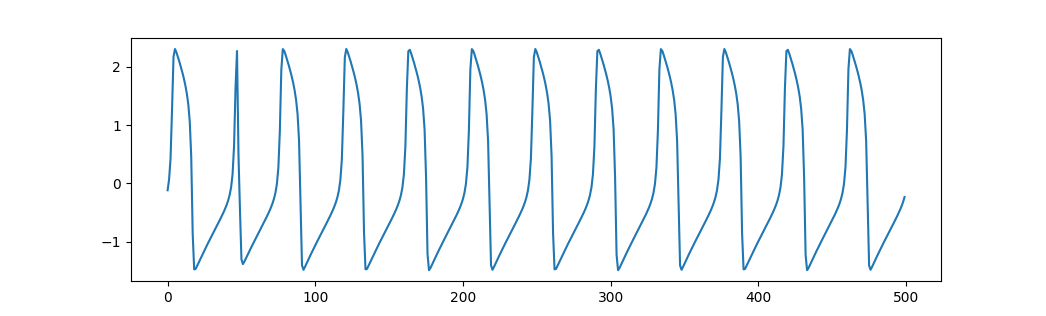
\includegraphics[width=0.9\linewidth]{fitzhughnagumo_sample.png}
  \caption[
    Sample time series based on the solution of the FitzHugh-Nagumo model
  ]
  {
    Sample time series based on the solution $v(t)$ of the FitzHugh-Nagumo model, with parameters
    $RI_{\mathrm{ext}}$ = 0.4, $\tau$ = 12.5, $a$ = 0.7, $b$ = 0.82.
  }
  \label{fig:fitzhughnagumo_sample}
\end{figure}

Biological time series, including the ones examined by this chapter, have noise.
To assess the affect of noise on the behaviour of models and on the cross-correlation function, I add noise to the models of oscillators.
I use two types of noise in my investigation: Gaussian noise and Gillespie noise.

Gaussian noise is the simple, first-approach case, and is generated by randomly drawing samples from the normal distribution $\mathcal{N}(0,\sigma^{2})$, where $\sigma$ denotes the standard deviation of the distribution and thus controls the size of the noise.

Gillespie noise emulates noise from biological systems and is generated using the direct method of the Gillespie algorithm \parencite{gillespieExactStochasticSimulation1977} on the birth-death process model.
The Gillespie algorithm was developed for stochastic simulations of a biochemical system.

(INSERT SHORT SUMMARY HERE AND LINK TO APPENDIX)

\begin{figure}
  \centering
  \begin{subfigure}{0.4\textwidth}
    \centering
    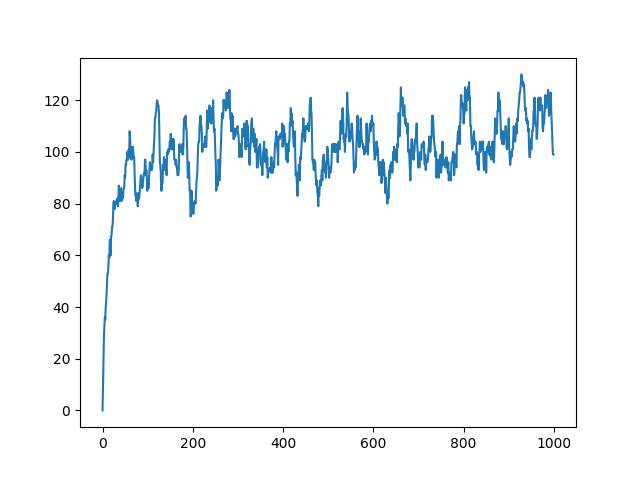
\includegraphics[width=\linewidth]{gillespie}
    \caption{
      Stochastic simulation of trajectory of $P$, as defined by the birth-death process with $k_{0} = 5$ and $d_{0} = 0.05$ (equation~\ref{eq:birth-death-process}), produced by the direct Gillespie algorithm.
      $t_{\mathrm{max}}$ in the simulation is \num{1500}, but the time points were then interpolated on a regular grid of \num{1000} time points.
    }
    \label{fig:gillespie_trajectory}
  \end{subfigure}

 \begin{subfigure}{0.9\textwidth}
    \centering
    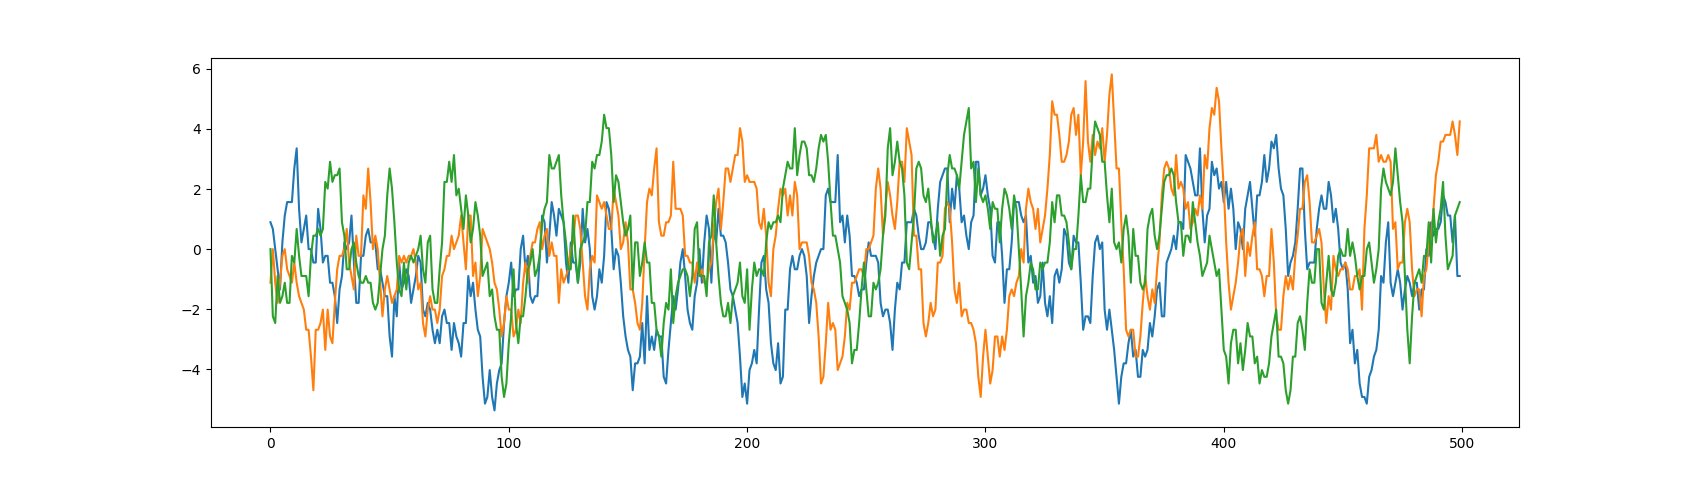
\includegraphics[width=\linewidth]{gillespie_noise_samples}
    \caption{
      Sample trajectories of Gillespie noise, produced from the latter half of trajectories as those shown in~\ref{fig:gillespie_trajectory}.
    }
    \label{fig:gillespie_noise_samples}
  \end{subfigure}

  \caption{Generation of Gillespie noise.}
  \label{fig:gillespie_noise}
\end{figure}

Gaussian or Gillespie noise was added to the synthetic oscillatory time series by computing element-wise sums.

\subsubsection{Effect of noise parameters on the autocorrelation function}
\label{subsubsec:analysis-characterisation-acf-sinusoid}

\begin{figure}
  \centering
  \begin{subfigure}[t]{0.45\textwidth}
  \centering
  % TODO: Replace with 3 sinusoids
    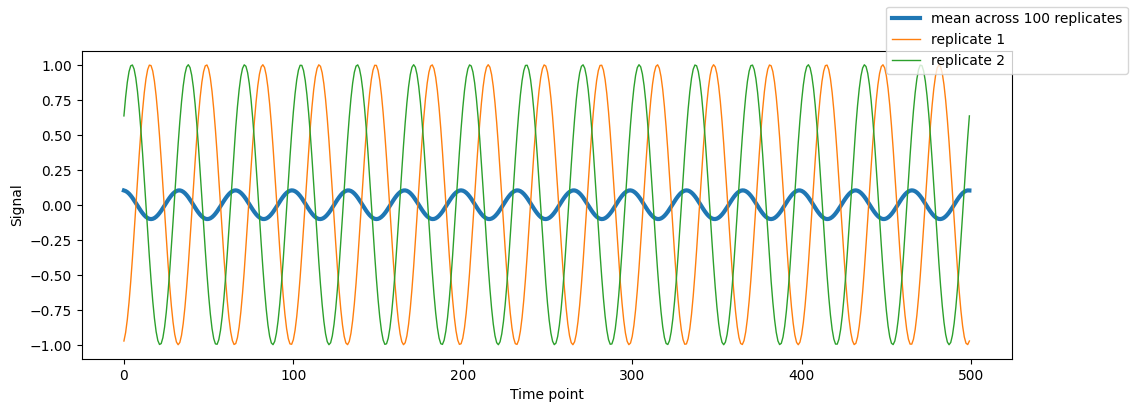
\includegraphics[width=\linewidth]{sinusoids_outofphase}
    \caption{
      400 out-of-phase sinusoids with frequency 0.03.
    }
    \label{fig:acf-sinusoids-nonoise-ts}
  \end{subfigure}%
  \centering
  \begin{subfigure}[t]{0.45\textwidth}
  \centering
    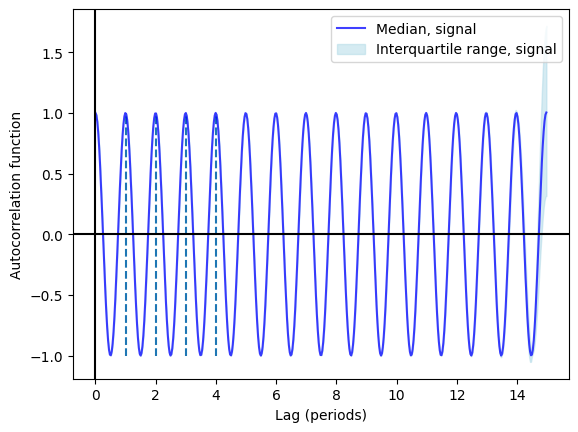
\includegraphics[width=\linewidth]{sinusoids_outofphase_acf_corrected}
    \caption{
      Autocorrelation function of~\ref{fig:acf-sinusoids-nonoise-ts}.
    }
    \label{fig:acf-sinusoids-nonoise-acf}
  \end{subfigure}

  % TODO: Use the (high) noise level quoted, and generate 3 sinusoids to replace this,
  % as above.
  \begin{subfigure}[t]{0.45\textwidth}
  \centering
    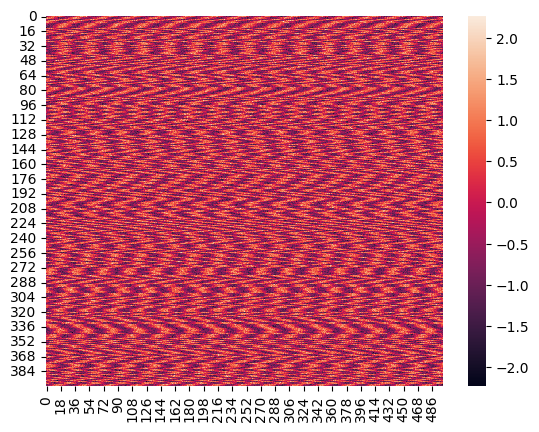
\includegraphics[width=\linewidth]{noisysinusoids_outofphase}
    \caption{
      400 out-of-phase sinusoids with frequency 0.03, each with Gaussian noise with a standard deviation of 3.
    }
    \label{fig:acf-sinusoids-gausnoise-ts}
  \end{subfigure}%
  \centering
  \begin{subfigure}[t]{0.45\textwidth}
  \centering
    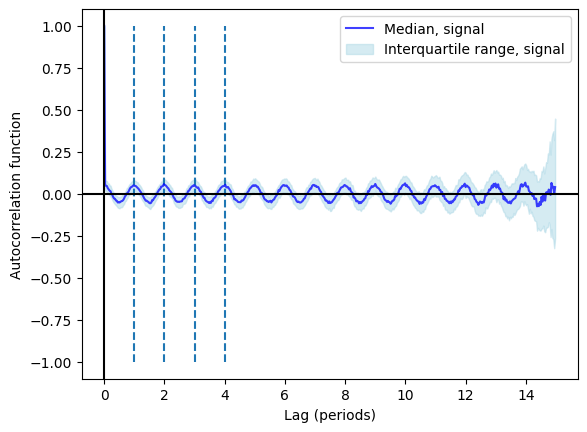
\includegraphics[width=\linewidth]{verynoisysinusoids_outofphase_acf}
    \caption{
      Autocorrelation function of~\ref{fig:acf-sinusoids-gausnoise-ts}.
    }
    \label{fig:acf-sinusoids-gausnoise-acf}
  \end{subfigure}

  \begin{subfigure}[t]{0.45\textwidth}
  \centering
    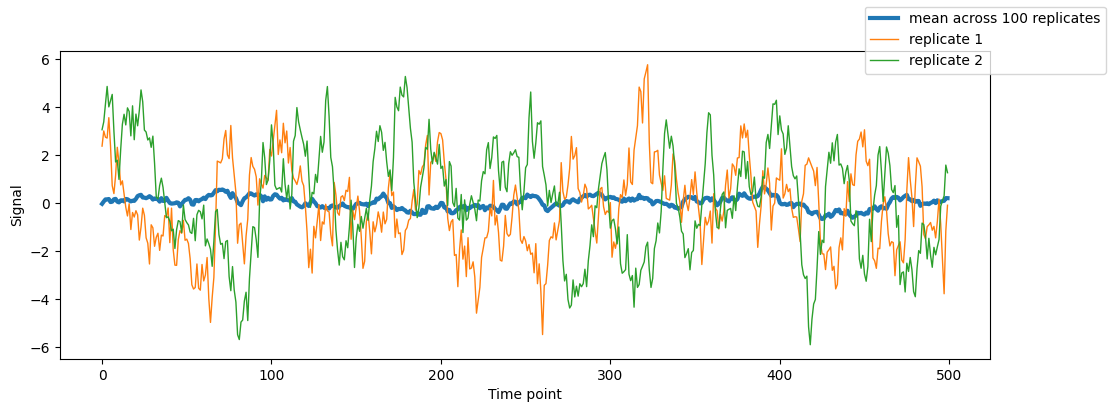
\includegraphics[width=\linewidth]{gillespie_k5_d0p05_mean}
    \caption{
      Sample sinusoids with frequency 0.03, each with Gillespie noise with $k_{0} = 5$ and $d_{0} = 0.05$.
    }
    \label{fig:acf-sinusoids-gillnoise-ts}
  \end{subfigure}%
  \centering
  \begin{subfigure}[t]{0.45\textwidth}
  \centering
    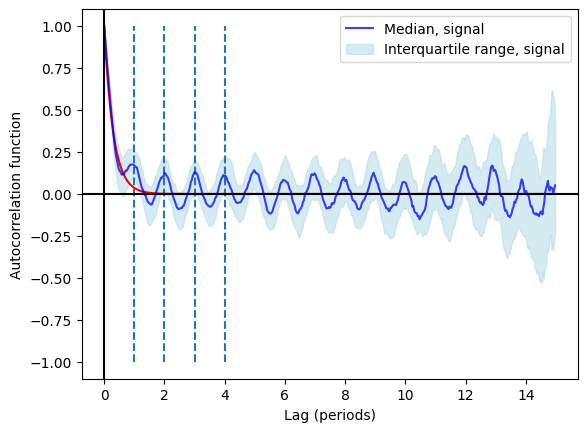
\includegraphics[width=\linewidth]{gillespie_k5_d0p05_acf}
    \caption{
      Autocorrelation function of~\ref{fig:acf-sinusoids-gillnoise-ts}.
      Red line is defined by $y = \me^{-2d_{0}T}$, where $T$ represents lag, which should in theory fit the median autocorrelation function.
    }
    \label{fig:acf-sinusoids-gillnoise-acf}
  \end{subfigure}

  \caption{
    Effect of type of noise on the autocorrelation function.
  }
  \label{fig:acf-sinusoids}
\end{figure}

To build understanding of the autocorrelation function on noisy time series, I start from the simple case of using the sinusoid as the input time series.

First, I generated a population of 400 out-of-phase sinusoids of the same frequency (figure~\ref{fig:acf-sinusoids-nonoise-ts}), and computed the autocorrelation function across the population (figure~\ref{fig:acf-sinusoids-nonoise-acf}).
The phase of each sinusoid was randomised, sampled from the uniform distribution \(Unif[0,2\pi)\).
As expected from the theoretical definitions, each autocorrelation function, corresponding to each time series, resembles a cosine with an amplitude of 1 and the same period as the sinusoids.
% [Show working -- i.e. the mathematical derivations that make me expect this?]

Second, to investigate the effect of Gaussian noise, I added Gaussian noise with standard deviation 3.0 (figure~\ref{fig:acf-sinusoids-gausnoise-ts}).
Here, the amplitude of the autocorrelation functions (figure~\ref{fig:acf-sinusoids-gausnoise-acf}) are decreased and the variation between each time series' autocorrelation function is increased.
At higher lag times, this variation is greater because there is fewer data that is used to compute the autocorrelation function.

Third and finally, to investigate the effect of Gillespie noise, I generated Gillespie noise using the birth-death process and parameters $k_{0} = 5$, $d_{0} = 0.05$, then added the noise to a population of 100 sinusoids, out-of-phase (figure~\ref{fig:acf-sinusoids-gillnoise-ts}).
The autocorrelation function is given by figure~\ref{fig:acf-sinusoids-gillnoise-acf}.
This gave the following mean across replicates and autocorrelation function.
% [Show working -- i.e. the mathematical derivations that make me expect this exponential fit?]
The exponential decay function $y = \me^{-2d_{0}T}$, where $T$ represents lag, should in theory fit the median autocorrelation function, and I demonstrate that it is the case.
In addition, the oscillations in the autocorrelation function should occur every period of the sinusoid, similar to the other noise cases.

\begin{figure}
  \centering
  \begin{subfigure}[t]{0.45\textwidth}
  \centering
    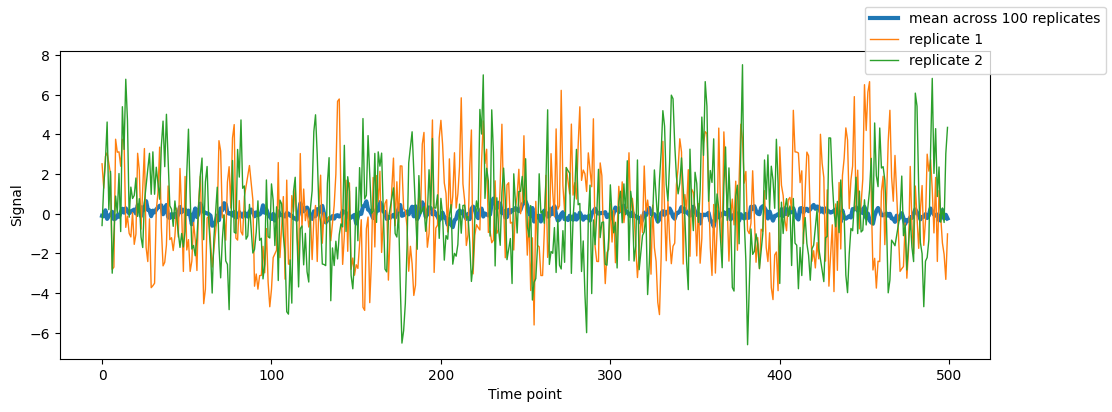
\includegraphics[width=\linewidth]{gillespie_k5_d0p5_mean.png}
    \caption{
      Sample sinusoids, with Gillespie noise ($k_{0} = 5$, $d_{0} = 0.5$).
    }
    \label{fig:acf-noisetimescale-highd0-ts}
  \end{subfigure}%
  \begin{subfigure}[t]{0.45\textwidth}
  \centering
    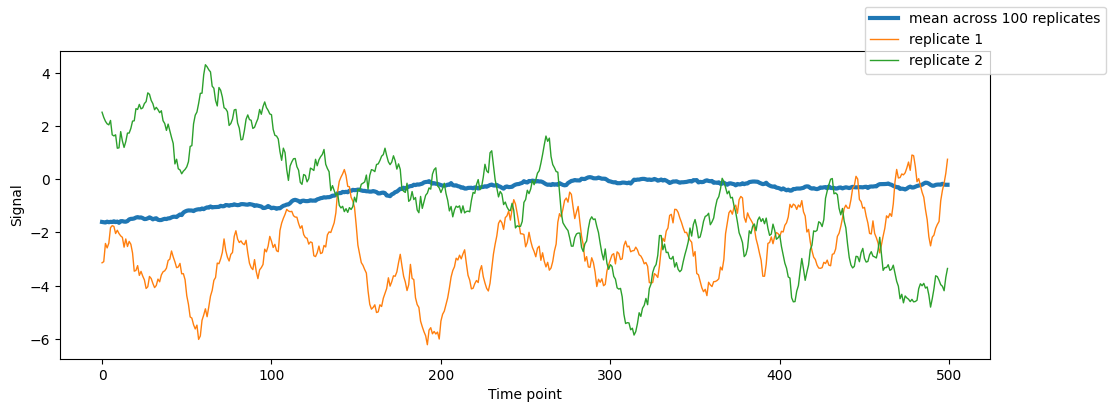
\includegraphics[width=\linewidth]{gillespie_k5_d0p005_mean.png}
    \caption{
      Sample sinusoids, with Gillespie noise ($k_{0} = 5$, $d_{0} = 0.005$).
    }
    \label{fig:acf-noisetimescale-lowd0-ts}
  \end{subfigure}

  \begin{subfigure}[t]{0.45\textwidth}
  \centering
    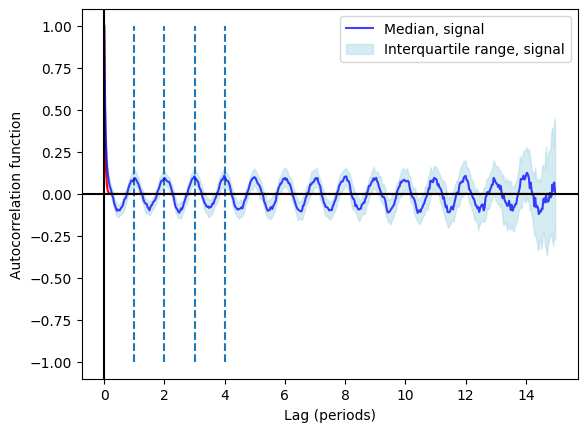
\includegraphics[width=\linewidth]{gillespie_k5_d0p5_acf.png}
    \caption{
      Autocorrelation function of~\ref{fig:acf-noisetimescale-highd0-ts}.
    }
    \label{fig:acf-noisetimescale-highd0-acf}
  \end{subfigure}%
  \begin{subfigure}[t]{0.45\textwidth}
  \centering
    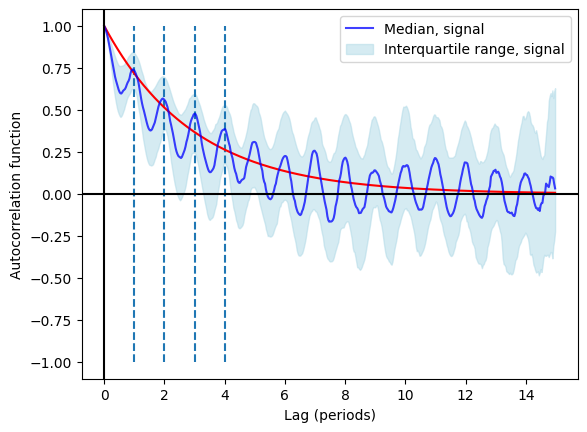
\includegraphics[width=\linewidth]{gillespie_k5_d0p005_acf.png}
    \caption{
      Autocorrelation function of~\ref{fig:acf-noisetimescale-lowd0-ts}.
    }
    \label{fig:acf-noisetimescale-lowd0-acf}
  \end{subfigure}

  \caption[
    Effect of death rate of Gillespie noise on the autocorrelation function.
  ]{
    Effect of death rate ($d_{0}$) of Gillespie noise on the autocorrelation function.
    Red lines on bottom figures (autocorrelation functions) are defined by $y = \me^{-2d_{0}T}$, where $T$ represents lag.
  }
  \label{fig:acf-noisetimescale}
\end{figure}

\begin{figure}
  \centering
  \begin{subfigure}[t]{0.45\textwidth}
  \centering
    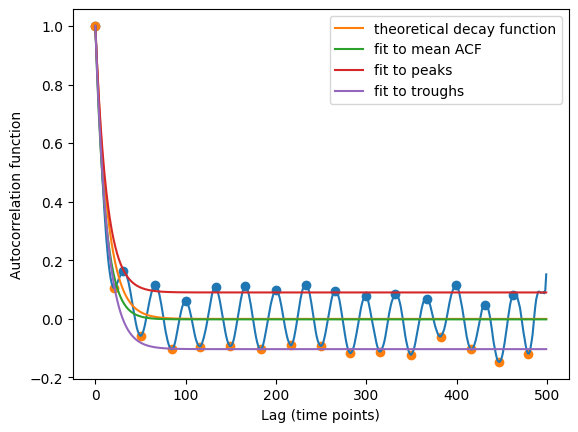
\includegraphics[width=\linewidth]{acf_fit_example.png}
    \caption{
      Exponential decay functions of the form $y = (1-C)\me^{-DT}+C$, with $C$ and $D$ as variable parameters, were fit to the mean autocorrelation function, the peaks of this mean function, and the troughs of these functions, using non-linear least squares.
    }
    \label{fig:acf-noisetimescale-effect-fit}
  \end{subfigure}%
  \begin{subfigure}[t]{0.45\textwidth}
  \centering
    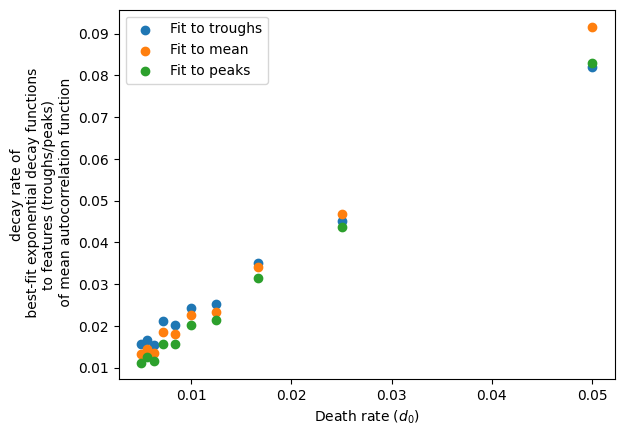
\includegraphics[width=\linewidth]{deathrate_vs_decay.png}
    \caption{
      The exponential fitting was performed across a range of $d_{0}$ while $k_{0}$ was held constant at 5.
      The decay rates $D$ of the exponential fits scale linearly with $d_{0}$.
    }
    \label{fig:acf-noisetimescale-effect-relationship}
  \end{subfigure}

  \caption{
    Characterising the autocorrelation function to quantify the effect of Gillespie noise timescale.
  }
  \label{fig:acf-noisetimescale-effect}
\end{figure}

It is now established that if the sinusoids have Gillespie noise, the noise parameters affect the shape of the autocorrelation function of the population of sinusoids.
Therefore, I investigate the effect of the timescale of noise and the amplitude of noise on the shape of the autocorrelation function.

To investigate the effect of the timescale of noise, defined by $\tau = 1/d_{0}$, I varied the death rate parameter $d_{0}$ when generating Gillespie noise that is to be added to the sinusoids (figure~\ref{fig:acf-noisetimescale}).
A higher death rate decreases the decay timescale of the autocorrelation function, while a lower death rate introduces long-term trends in the simulated signals.
A lower death rate also increases the decay timescale for the autocorrelation function and increases the variation between autocorrelation functions between replicates.
In theory, the decay rate $D$ of the autocorrelation function should scale linearly with the death rate $d_{0}$.
To confirm this, I fit exponential decay functions of the form $y = (1-C)\me^{-DT}+C$ to the mean autocorrelation, the peaks of this mean function, and the troughs of these functions using non-linear least squares fitting (figure~\ref{fig:acf-noisetimescale-effect-fit}).
Then, I found the best-fit parameter $D$ for each value of $d_{0}$ (figure~\ref{fig:acf-noisetimescale-effect-relationship}).
In sum, the death rate $d_{0}$ controls the decay rate $D$ of the autocorrelation function; conversely, if $D$ can be estimated from the autocorrelation function, then the noise timescale $\tau$ of the time series can be estimated.


\begin{figure}
  \centering
  \begin{subfigure}[t]{0.45\textwidth}
  \centering
    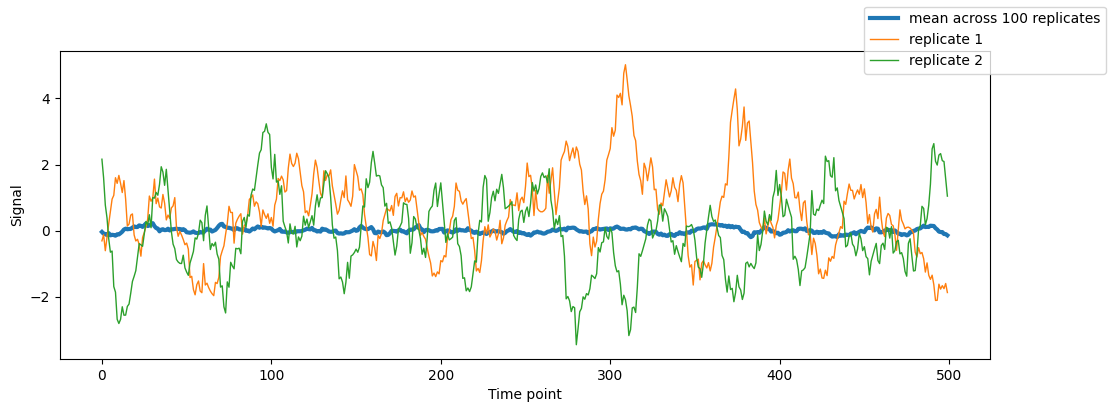
\includegraphics[width=\linewidth]{gillespie_k1_d0p05_mean.png}
    \caption{
      Sample sinusoids, with Gillespie noise ($k_{0} = 1$, $d_{0} = 0.05$).
    }
    \label{fig:acf-noiseamplitude-lowk0-ts}
  \end{subfigure}%
  \begin{subfigure}[t]{0.45\textwidth}
  \centering
    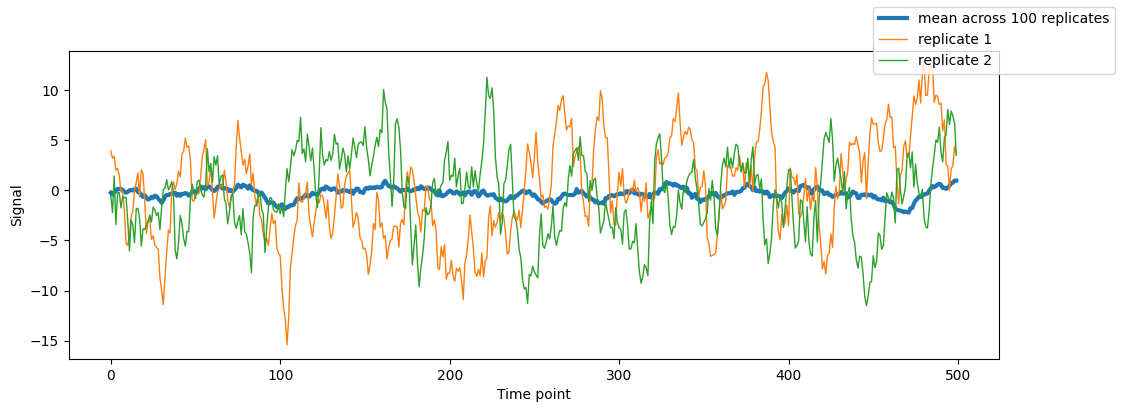
\includegraphics[width=\linewidth]{gillespie_k25_d0p05_mean.png}
    \caption{
      Sample sinusoids, with Gillespie noise ($k_{0} = 25$, $d_{0} = 0.05$).
    }
    \label{fig:acf-noiseamplitude-highk0-ts}
  \end{subfigure}

  \begin{subfigure}[t]{0.45\textwidth}
  \centering
    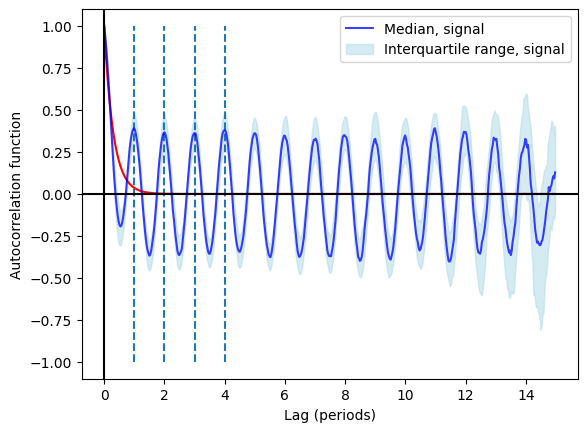
\includegraphics[width=\linewidth]{gillespie_k1_d0p05_acf.png}
    \caption{
      Autocorrelation function of~\ref{fig:acf-noiseamplitude-lowk0-ts}.
    }
    \label{fig:acf-noiseamplitude-lowk0-acf}
  \end{subfigure}%
  \begin{subfigure}[t]{0.45\textwidth}
  \centering
    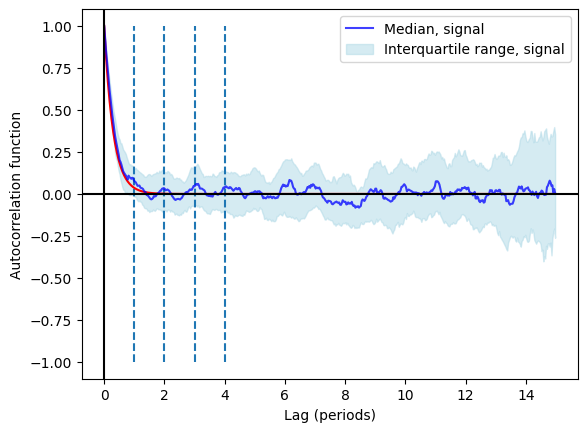
\includegraphics[width=\linewidth]{gillespie_k25_d0p05_acf.png}
    \caption{
      Autocorrelation function of~\ref{fig:acf-noiseamplitude-highk0-ts}.
    }
    \label{fig:acf-noiseamplitude-highk0-acf}
  \end{subfigure}

  \caption[
    Effect of birth rate of Gillespie noise on the autocorrelation function.
  ]{
    Effect of birth rate ($k_{0}$) of Gillespie noise on the autocorrelation function.
    Red lines on bottom figures (autocorrelation functions) are defined by $y = e^{-2d_{0}T}$, where $T$ represents lag.
  }
  \label{fig:acf-noiseamplitude}
\end{figure}

\begin{figure}
  \centering
  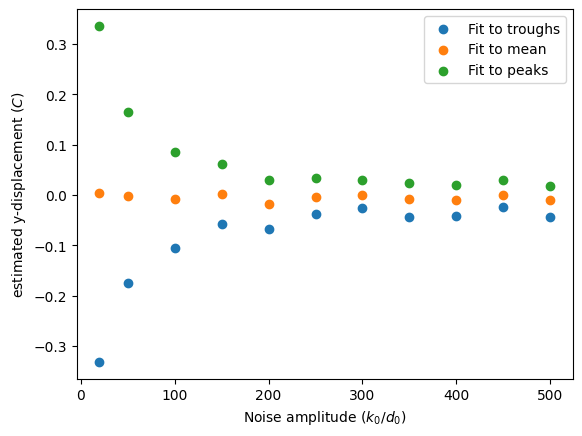
\includegraphics[width=0.6\linewidth]{birthrate_vs_ydispl.png}
  \caption[
    Quantifying the effect of Gillespie noise amplitude on the autocorrelation function
  ]{
    Quantifying the effect of Gillespie noise amplitude on the autocorrelation function.
    Exponential decay functions of the form $y = (1-C)e^{-DT}+C$, with $C$ and $D$ as variable parameters, were fit to the mean autocorrelation function, the peaks of this mean function, and the troughs of these functions, using non-linear least squares (as in~\ref{fig:acf-noisetimescale-effect-fit}).
    The exponential fitting was performed across a range of $k_{0}$ while $d_{0}$ was held constant at 0.05.
  }
  \label{fig:acf-noiseamplitude-effect}
\end{figure}


To investigate the effect of the amplitude of noise, defined by $A = \sqrt{k_{0}/d_{0}}$, I varied the birth rate parameter $k_{0}$ while keeping the death rate parameter $d_{0}$ constant when generating Gillespie noise that is to be added to the sinusoids (figure~\ref{fig:acf-noiseamplitude}).
A lower birth rate decreases the amplitude of noise.
It also makes the autocorrelation function more robust --- in other words, it decreases the variation between replicates.
Conversely, a higher birth rate increases the amplitude of noise.
It also makes the autocorrelation function less robust and increases the variation between replicates.
Similar to previously, I fit exponential decay functions of the form $y = (1-C)\me^{-DT}+C$ to the autocorrelation function, but now I find the best-fit values of the y-displacement parameter $C$ with respect to $k_{0}/d_{0}$ (figure~\ref{fig:acf-noiseamplitude-effect}).
The y-displacements $C$ of the exponential fits to peaks and troughs converged to 0 as the noise amplitude $k_{0}/d_{0}$ increased, showing that the amplitude of the oscillations in the autocorrelation function decreases as the noise amplitude increases.
In sum, the birth rate $d_{0}$ controls the y-displacement parameter $C$ of the autocorrelation function, which is a proxy for the function's amplitude.
Conversely, if $C$ can be estimated from the autocorrelation function, then the noise amplitude $A$ of the time series can be estimated.

To conclude, if a population of replicate oscillatory time series is modelled with the sum of sinusoids and Gillespie noise, then the birth rate and death rate can control the shape of the autocorrelation function.
The death rate controls the timescale of noise and thus how fast the autocorrelation decays as lag increases.
The birth rate controls the amplitude of noise and thus controls how robust the autocorrelation function is.


\begin{figure}
  \centering
  \begin{subfigure}[t]{0.7\textwidth}
  \centering
    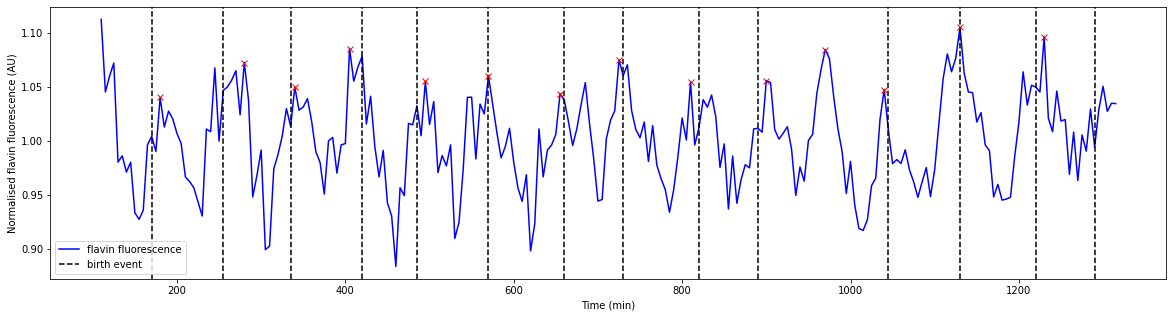
\includegraphics[width=\linewidth]{26643_ts.png}
    \caption{
      Sample time series of flavin autofluorescence.
    }
    \label{fig:acf-sinusoid-biol-ts}
  \end{subfigure}

  \begin{subfigure}[t]{0.7\textwidth}
  \centering
    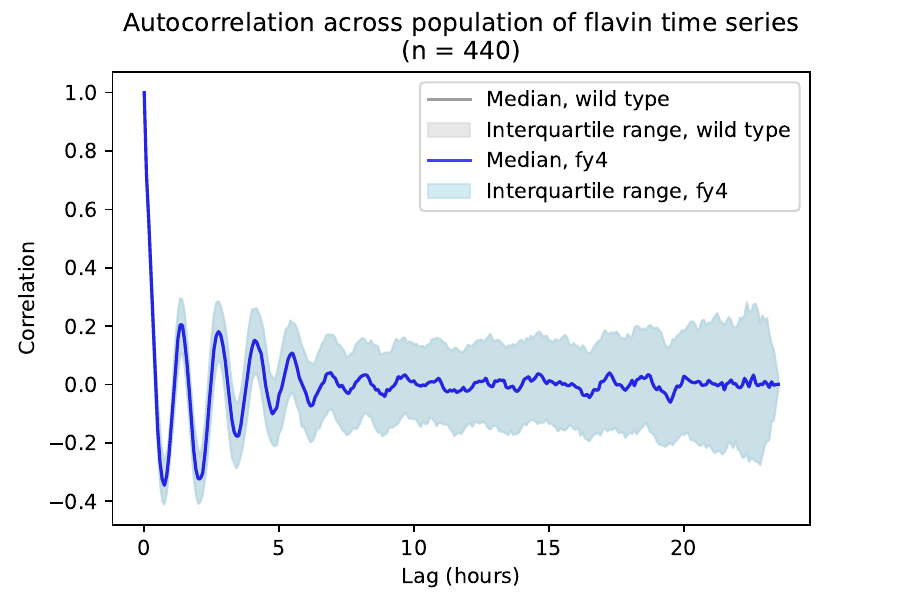
\includegraphics[width=\linewidth]{fy4_26643_plots_06.png}
    \caption{
      Autocorrelation function across a population of time series of flavin autofluorescence.
    }
    \label{fig:acf-sinusoid-biol-acf}
  \end{subfigure}

  \caption{
    Using the autocorrelation function to characterise oscillations in flavin autofluorescence.
  }
  \label{fig:acf-sinusoid-biol}
\end{figure}

Knowing these relationships, one can deduce noise parameters from the autocorrelation functions of real signals.
My intention is to have it model oscillations of flavin fluorescence that act as a proxy for the yeast metabolic cycle (figure~\ref{fig:acf-sinusoid-biol}).


\subsubsection{The autocorrelation function extended for use with FitzHugh-Nagumo oscillators}
\label{subsubsec:analysis-characterisation-acf-fhn}

Subsequently, I aim to extend the use of the autocorrelation function in quantifying the noise parameters of oscillatory signals from sinusoid signals to signals modelled by the FitzHugh-Nagumo oscillator.

\begin{figure}
  \centering
  \begin{subfigure}[t]{0.7\textwidth}
  \centering
    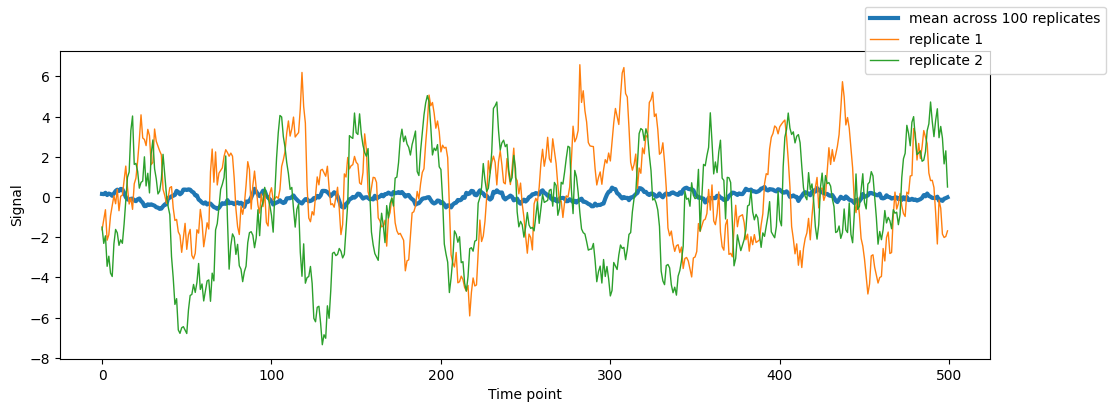
\includegraphics[width=\linewidth]{fhn_meanplot}
    \caption{
      Sample FitzHugh-Nagumo oscillators generated with parameters $RI_{\mathrm{ext}}$ = 0.4, $\tau$ = 12.5, $a$ = 0.7, $b$ = 0.82.
      Each was added with Gillespie noise generated with parameters $k_{0} = 5$ and $d_{0} = 0.05$.
    }
    \label{fig:acf-fhn-gillnoise-ts}
  \end{subfigure}

  \begin{subfigure}[t]{0.6\textwidth}
  \centering
    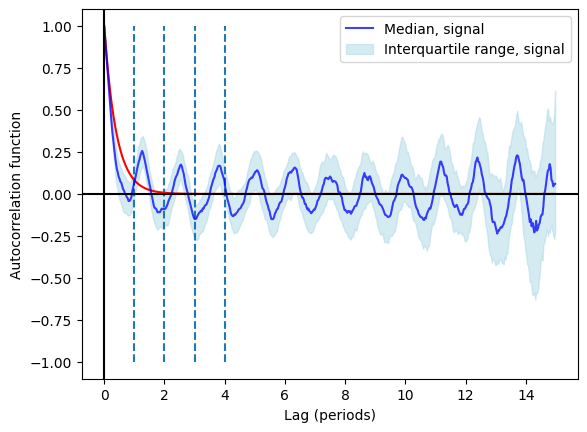
\includegraphics[width=\linewidth]{fhn_acf}
    \caption{
      Autocorrelation function of~\ref{fig:acf-fhn-gillnoise-ts}.
      Red line is defined by $y = \me^{-2d_{0}T}$, where $T$ represents lag.
    }
    \label{fig:acf-fhn-gillnoise-acf}
  \end{subfigure}

  \caption{
    The autocorrelation function of FitzHugh-Nagumo oscillators with Gillespie noise.
  }
  \label{fig:acf-fhn}
\end{figure}

\begin{figure}
  \centering
  \begin{subfigure}[t]{0.45\textwidth}
  \centering
    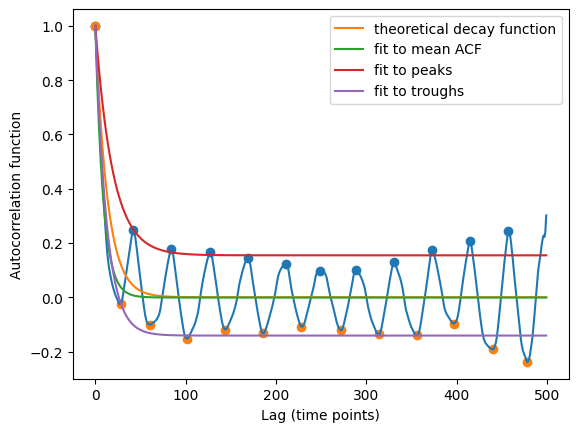
\includegraphics[width=\linewidth]{fhn_expofit}
    \caption{
      Exponential decay functions of the form $y = (1-C)\me^{-DT}+C$, with $C$ and $D$ as variable parameters, were fit to the mean autocorrelation function, the peaks of this mean function, and the troughs of these functions, using non-linear least squares.
    }
    \label{fig:acf-fhn-noiseparams-fit}
  \end{subfigure}%
  \begin{subfigure}[t]{0.45\textwidth}
  \centering
    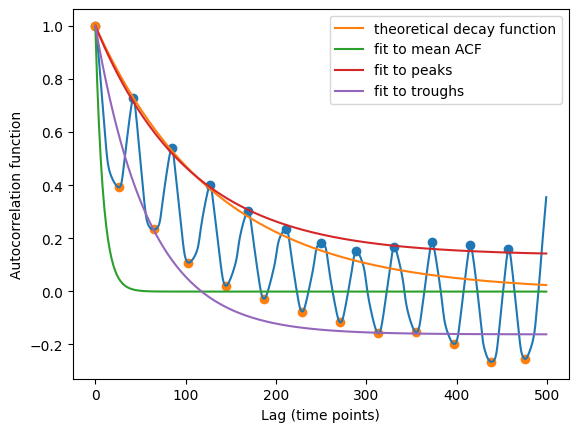
\includegraphics[width=\linewidth]{fhn_highnts_expofit}
    \caption{
      Similar to figure~\ref{fig:acf-fhn-noiseparams-fit}, but with a greater noise timescale, showing the limitations of this fitting with data using the FitzHugh-Nagumo oscillator as a base.
    }
    \label{fig:acf-fhn-noiseparams-fit-highnts}
  \end{subfigure}

  \begin{subfigure}[t]{0.45\textwidth}
  \centering
    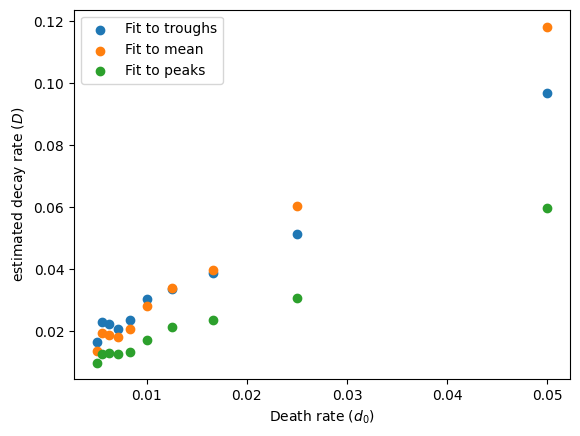
\includegraphics[width=\linewidth]{fhn_deathrate_vs_decay.png}
    \caption{
      The exponential fitting was performed across a range of $d_{0}$ while $k_{0}$ was held constant at 5.
      The decay rates $D$ of the exponential fits scale linearly with $d_{0}$.
    }
    \label{fig:acf-fhn-noiseparams-noisetimescale}
  \end{subfigure}%
  \begin{subfigure}[t]{0.45\textwidth}
  \centering
    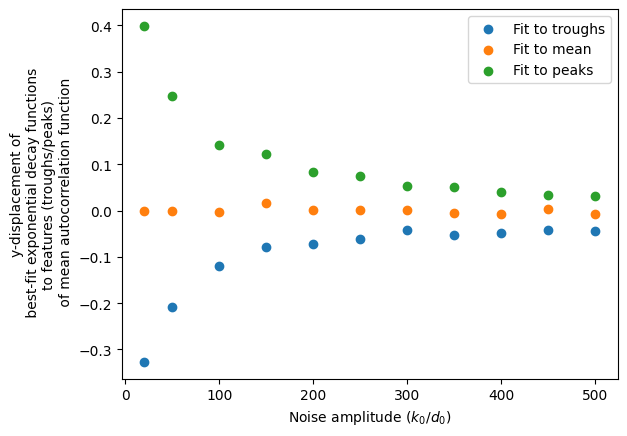
\includegraphics[width=\linewidth]{fhn_birthrate_vs_ydispl.png}
    \caption{
      The exponential fitting was performed across a range of $k_{0}$ while $d_{0}$ was held constant at 0.05.
      The y-displacements $C$ of the exponential fits to peaks and troughs converged to 0 as the noise amplitude $k_{0}/d_{0}$ increased, showing that the amplitude of the oscillations in the autocorrelation function decreases as the noise amplitude increases.
    }
    \label{fig:acf-fhn-noiseparams-noiseamplitude}
  \end{subfigure}

  \caption{
    Quantifying the effect of Gillespie noise parameters on the autocorrelation function of FitzHugh-Nagumo oscillators.
  }
  \label{fig:acf-fhn-noiseparams}
\end{figure}

My investigation used the same methods as in the previous section (\ref{subsubsec:analysis-characterisation-acf-sinusoid}).
Notably, the shape of the autocorrelation function of FitzHugh-Nagumo oscillators with Gillespie noise differed slightly to the sinusoid case --- namely, the waves are more pointed (figure~\ref{fig:acf-fhn-gillnoise-acf}).
In addition, fitting the exponential decay function $y = \me^{-2d_{0}T}$ to the autocorrelation function was less reliable, particularly with high noise timescales (figure~\ref{fig:acf-fhn-noiseparams-fit-highnts}).
As a consequence, estimating the noise timescale $\tau$ from the decay rate $D$ of the exponential decay function produces a greater range of uncertainty (figure~\ref{fig:acf-fhn-noiseparams-noisetimescale}).
However, estimating the noise amplitude $A$ based on the y-displacement $C$ of the exponential decay function remains as reliable as the sinusoid oscillator case (figure~\ref{fig:acf-fhn-noiseparams-noiseamplitude}).

\begin{figure}
  \centering
  \begin{subfigure}[t]{0.9\textwidth}
  \centering
  % TODO: Edit out the flavin bits
    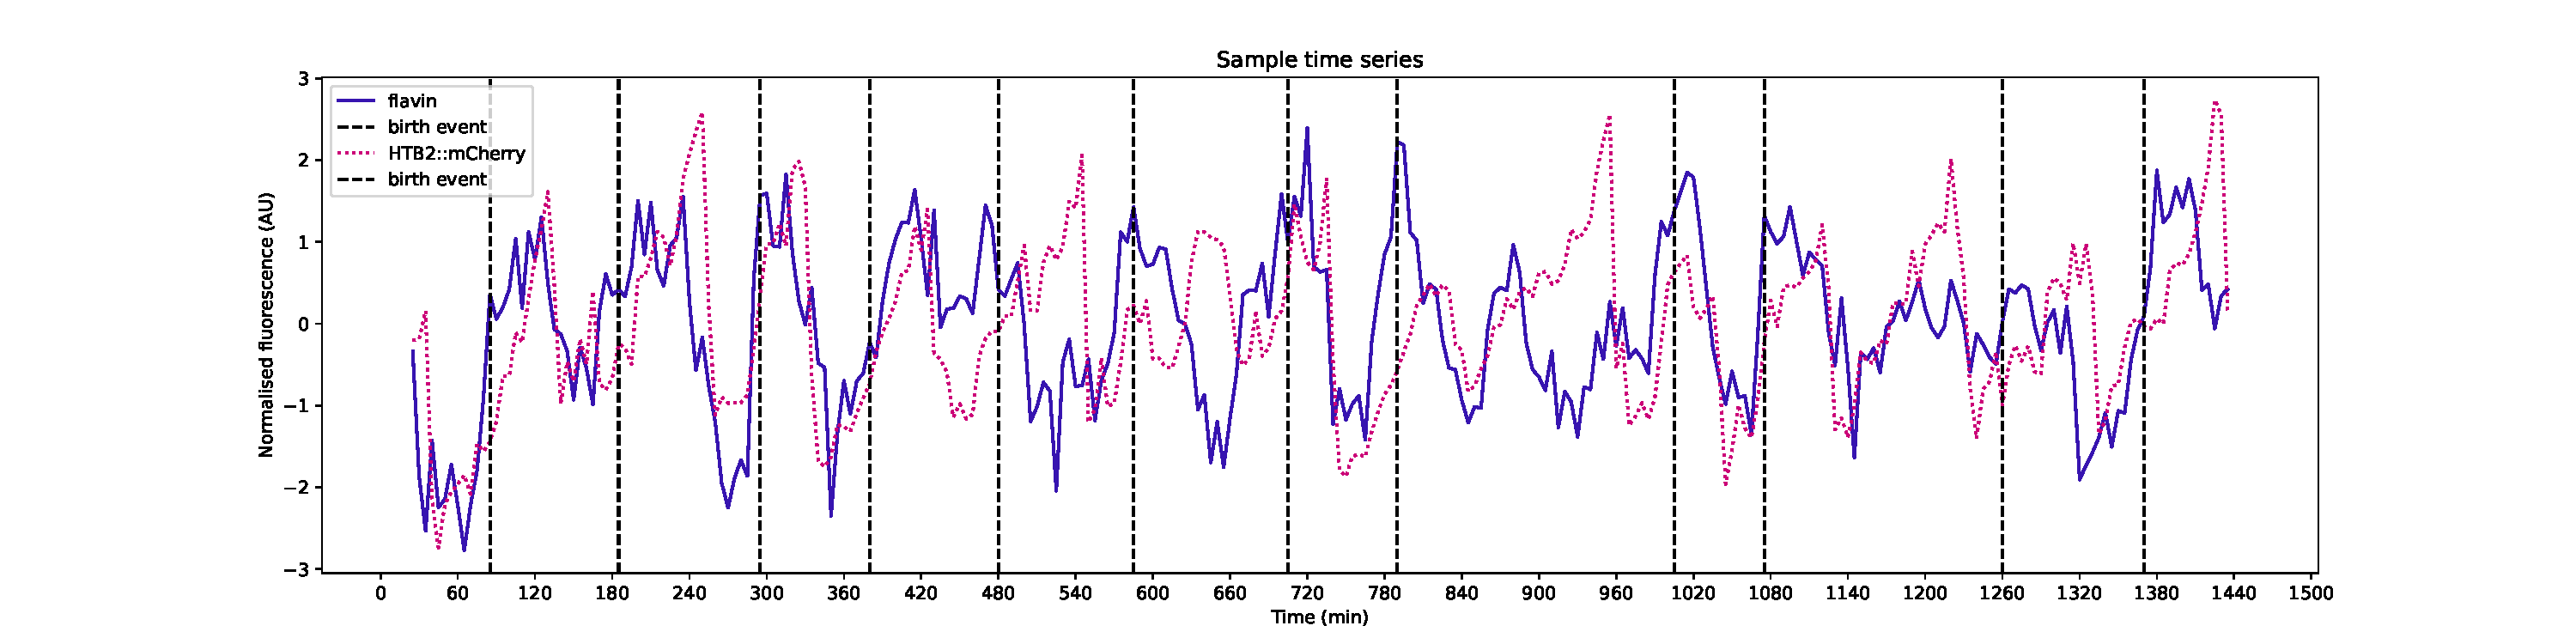
\includegraphics[width=\linewidth]{htb2mCherry_26643_plots_purple_01.pdf}
    \caption{
      Sample time series of histone 2B abundance (pink).
    }
    \label{fig:acf-fhn-biol-ts}
  \end{subfigure}

  \begin{subfigure}[t]{0.7\textwidth}
  \centering
    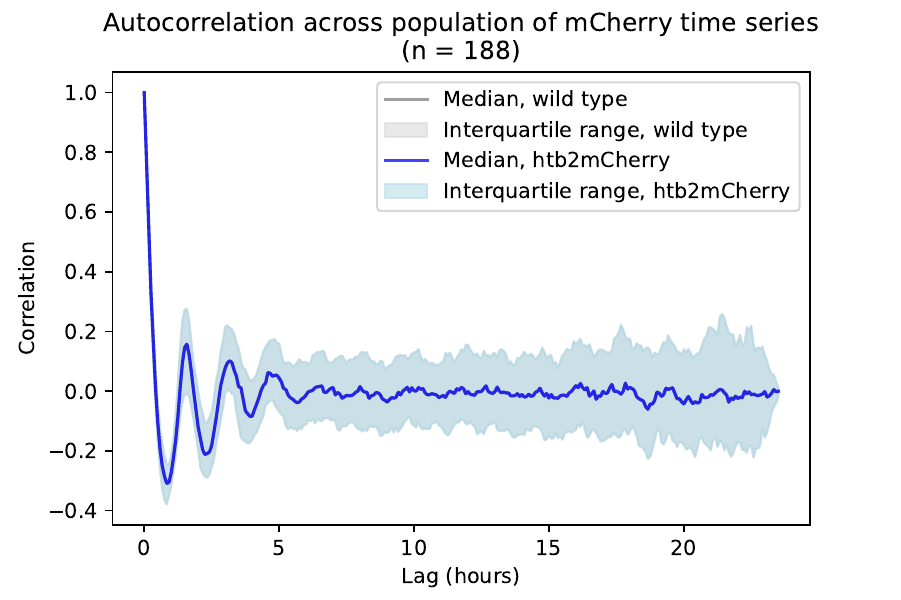
\includegraphics[width=\linewidth]{htb2mCherry_26643_plots_mCh_06.png}
    \caption{
      Autocorrelation function across a population of time series of histone 2B abundance.
    }
    \label{fig:acf-fhn-biol-acf}
  \end{subfigure}

  \caption{
    Using the autocorrelation function to characterise oscillations in histone 2B abundance.
  }
  \label{fig:acf-fhn-biol}
\end{figure}

My intention is to have the FitzHugh-Nagumo oscillator model periodic changes in histone 2B intensity levels and yeast cells progress through the cell division cycle (figure~\ref{fig:acf-fhn-biol}).


\subsection{Combining methods to get a picture of periodicity}
\label{subsec:analysis-characterisation-combined}

\begin{figure}
  \centering
  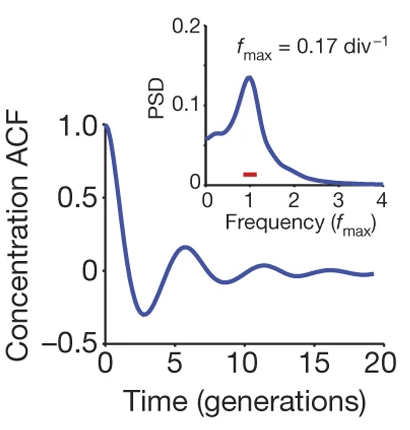
\includegraphics[width=0.5\linewidth]{potvin-trottierSynchronousLongtermOscillations2016_1e_adapted}
  \caption[
    Autocorrelation function and power spectral density calculated time series of cellular YFP concentration
  ]{
    Autocorrelation function (main) and power spectral density (upper-right inset) calculated over \num{8694} cell divisions' worth of time series of cellular YFP concentration controlled by a YFP-expressing repressilator.
    From the autocorrelation function, the average period of the oscillations is 5.6 generations, and the peak frequency of the power spectral density agrees.
    Adapted from \textcite{potvin-trottierSynchronousLongtermOscillations2016}.
  }
  \label{fig:acf-fft-example}
\end{figure}

As each method comes with own advantages and limitations --- especially apparent with noisy biological data --- it is useful to use several methods in concert get an idea of the periodicity of the oscillations, or other properties.
For example, \textcite{potvin-trottierSynchronousLongtermOscillations2016} combines the autocorrelation function and the Fourier transform to study the changes in the periodicity of a modified model of the repressilator (figure~\ref{fig:acf-fft-example}).
Thus, in my subsequent analysis of biological data, I combine the autocorrelation function and the Fourier spectrum.

% [FIGURE: SHOWS A GOOD TIME SERIES, FFT, ACF, AR, AND THE MOST PROBABLY OSCILLATION FREQUENCY FROM EACH]

% [FIGURE: THE SAME AS ABOVE BUT LOOKING AT A POPULATION OF TIME SERIES.  THESE TRAJECTORIES SHOULD HAVE BEEN COMPUTED INDIVIDUALLY FOR EACH TIME SERIES.  THE CAPTION SHOULD EXPLAIN THE MEAN/MEDIAN AND ERROR RANGES.]

\subsection{New subsection for noise}
\label{subsec:analysis-characterisation-noise}

\begin{figure}
  \centering
  \begin{subfigure}[htpb]{0.5\textwidth}
   \centering
   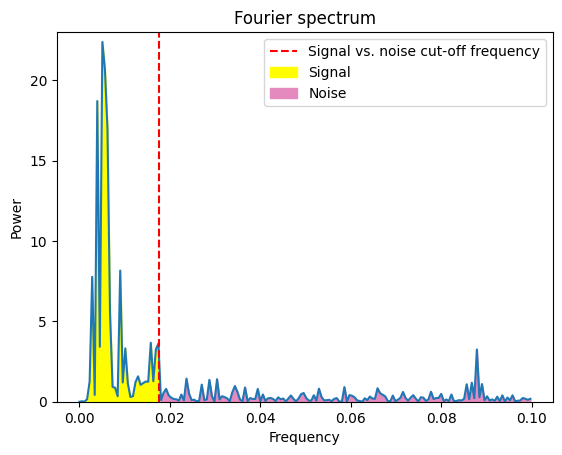
\includegraphics[width=\textwidth]{snr_illustration}
   \caption{
     To define the signal-to-noise ratio, a cut-off frequency is defined to divide the area under the Fourier spectrum: signal, to the left of the cut-off (yellow), and noise, to the right (pink).
     The signal-to-noise ratio is thus defined as the signal area divided by the noise area.
   }
   \label{fig:analysis-snr-illustration}
 \end{subfigure}%
 \begin{subfigure}[htpb]{0.5\textwidth}
   \centering
   \includegraphics[width=\textwidth]{pyruvate_snr_edit}
   \caption{
     The signal-to-noise ratio was computed for each processed signal within a dataset, and the distribution of these ratios within a dataset can indicate the overall quality of signals.
   }
   \label{fig:analysis-snr-histogram-example}
  \end{subfigure}
  \caption{
    The signal-to-noise ratio as a measure of signal quality.
  }
  \label{fig:analysis-snr}
\end{figure}

Finally, I discuss a way to evaluate the quality of a (processed) dataset --- specifically, computing a signal-to-noise ratio.
The signal-to-noise ratio compares the level of a desired signal to background noise and serves as a measure of quality in signal processing.
It takes various definitions depending on how the signal and noise are defined.
In my case, I base my definition on the frequency domain of the signal.
I define a cut-off frequency between signal and noise (figure~\ref{fig:analysis-snr}), based on the assumption that very high-frequency components of the periodogram correspond to noise and lower-frequency components correspond to the meaningful oscillations.% (and this is after filtering out the very low-frequency components that are the long-term trends I don't want).
Again, this is a judgement call, and this is based on looking at several experiments' mean Fourier spectrum and defining a number that best separates signal and noise.

%[EVIDENCE NEEDED -- PERHAPS PLOTS FROM SEVERAL EXPERIMENTS THAT PRODUCE DIFFERENT-FREQUENCY OSCILLATIONS.  OR THE MEAN FOURIER SPECTRUM OF SOME EXPERIMENT, OVERLAID WITH THE CUT-OFF LINE.]

To summarise, choosing relevant and `clean' data is needed for all data pipelines, but time series data expected to be oscillatory needs filtering or detrending to separate the oscillations of interest from irrelevant trends in the data.
For my data, I choose cells whose tracks are present for at least 80\% of the experiment, interpolate missing time points, and use a high-pass Butterworth filter with a critical frequency of \SI[parse-numbers=false]{1/350}{\minute^{-1}} to remove long-term trends and to preserve noise for quality evaluation using the signal-to-noise ratio measure.


\section[Correlation]{Correlation: I have two signals from the same cell --- what are their relationships to each other?}
\label{sec:analysis-correlation}

So far, I have considered one type of time series from the yeast metabolic oscillator at a time.
However, the yeast metabolic oscillator and the cell division cycle form part of a system of coupled oscillators
In my experiments I record signals that monitor both.
Investigating correlations between two paired time series, originating from the same cell, leads to an understanding of the relationship between the two oscillators.
The most important being the phase relationship: does one oscillation lag behind the other, to what extent, and is this consistent across cells?

% [COMMENTED OUT BECAUSE IT IS THE SOLE SUBSECTION]
% \subsection{Cross-correlation}
% \label{subsec:analysis-correlation-xcf}

In signal processing, cross-correlation is used to measure how similar two time series are, as the displacement of one relative to the other is shifted across the length of the time series.
In a biological context, cross-correlation has been used to investigate the relationship between the expression levels of two genes in a model feed-forward loop \parencite{dunlopRegulatoryActivityRevealed2008},
and to investigate the relationship between instantaneous growth rate and the expression of \textit{lac} genes OR of enzymes in central metabolism across a population of \textit{E. coli} cells \parencite{kivietStochasticityMetabolismGrowth2014}.
Importantly, \textcite{kivietStochasticityMetabolismGrowth2014} employs a single-cell microfluidics experiment with time-lapse microscopy, and therefore their treatment of a population of time series is useful for my case.
Therefore, my use of cross-correlation is adapted from theirs so that it suits a population of time series.
My implementation has already been described in section~\ref{subsubsec:analysis-characterisation-acf-maths}.

As in my discussion of autocorrelation (section~\ref{subsec:analysis-characterisation-acf}), I will start with the sinusoid and FitzHugh-Nagumo oscillators as simulations of my biological time series to show understanding of the methods, then apply the understand to a real dataset.

\begin{figure}
  \centering
  \begin{subfigure}[t]{0.45\textwidth}
  \centering
  % TODO: Squish so that it is consistent with adjacent figure
    \includegraphics[width=\linewidth]{sinusoid_and_fitzhughnagumo_nonoise.png}
    \caption{
      Sample FitzHugh-Nagumo oscillator (orange) generated with parameters $RI_{\mathrm{ext}}$ = 0.4, $\tau$ = 12.5, $a$ = 0.7, $b$ = 0.82, and a sinusoid of frequency 0.026 (blue), adjusted so that its frequency is the same as that of the FitzHugh-Nagumo oscillator.
    }
    \label{fig:xcf-nonoise-ts}
  \end{subfigure}%
  \centering
  \begin{subfigure}[t]{0.45\textwidth}
  \centering
    \includegraphics[width=\linewidth]{randomshift_sinusoid_fitzhughnagumo_xcf.png}
    \caption{
      Cross-correlation function of the FitzHugh-Nagumo oscillator with respect to the sinusoid oscillator, based on 400 pairs of signal as in~\ref{fig:xcf-nonoise-ts}, each pair randomly phase-shifted.
    }
    \label{fig:xcf-nonoise-xcf}
  \end{subfigure}

  % TODO: Use Gillespie noise.  Maybe this figure already exists.
  \begin{subfigure}[t]{0.45\textwidth}
  \centering
    \includegraphics[width=\linewidth]{sinusoid_and_fitzhughnagumo_gillnoise.png}
    \caption{
      FitzHugh-Nagumo (orange) and sinusoid oscillators (blue), as in~\ref{fig:xcf-nonoise-ts}, but with Gillepsie noise ($d_{0} = 0.05$, $k_{0} = 5$).
    }
    \label{fig:xcf-gillnoise-ts}
  \end{subfigure}%
  \centering
  \begin{subfigure}[t]{0.45\textwidth}
  \centering
    \includegraphics[width=\linewidth]{randomshift_sinusoid_fitzhughnagumo_gillnoise_xcf.png}
    \caption{
      Cross-correlation function of the FitzHugh-Nagumo oscillator with respect to the sinusoid oscillator, based on 400 pairs of signal as in~\ref{fig:xcf-gillnoise-ts}, each pair randomly phase-shifted.
    }
    \label{fig:xcf-gillnoise-xcf}
  \end{subfigure}

  \caption{
    Using the cross-correlation function to evaluate the shift of one synthetic time series relative to another with a different shape.
  }
  \label{fig:xcf}
\end{figure}

First, I generated a population of 400 FitzHugh-Nagumo oscillators and a population of 400 sinusoids so that they have the same period as the FitzHugh-Nagumo oscillator, but shifted in phase (figure~\ref{fig:xcf-nonoise-ts}).
This simulates flavin autofluorescence oscillations and oscillations in histone 2B abundance both being at the same frequency, owing to the coupling between the metabolic cycle and the cell division cycle, but may be out of phase.
The cross-correlation function of each FitzHugh-Nagumo oscillator with respect to the sinusoid oscillator, across the population, was computed (figure~\ref{fig:xcf-nonoise-xcf}).
If the two types of oscillators are in phase (i.e.\ the peaks coincide), the cross-correlation at lag 0 should be 1.
However, as the two oscillators are shifted in phase relative to each other, this peak of the cross-correlation function is shifted to the right, and the $x$-position of this peak thus indicates the average time by which the FitzHugh-Nagumo oscillator is shifted forward relative to the sinusoid oscillator, across the population.
As before, I added noise (figure~\ref{fig:xcf-gillnoise-ts}) to investigate the effect on the cross-correlation function (figure~\ref{fig:xcf-gillnoise-xcf}).
This illustrates that the cross-correlation function can still find phase relationships between two types of oscillatory data, even if the noise is extreme.

% TODO: Replace with pyruvate?  More dramatic.
\begin{figure}
  \centering
  \begin{subfigure}[t]{0.9\textwidth}
  \centering
    \includegraphics[width=\linewidth]{htb2mCherry_26643_plots_purple_01.pdf}
    \caption{
      Sample time series of flavin autofluorescence (purple) and histone 2B abundance (pink).
    }
    \label{fig:xcf-biol-ts}
  \end{subfigure}

  \begin{subfigure}[t]{0.7\textwidth}
  \centering
    \includegraphics[width=\linewidth]{xcf_edit.pdf}
    \caption{
      Cross-correlation function of the histone 2B abundance time series with respect to the flavin autofluorescence time series.
    }
    \label{fig:xcf-biol-xcf}
  \end{subfigure}

  \caption{
    Using the cross-correlation function to evaluate the shift of histone 2B abundance traces with respect to flavin autofluorescence traces.
  }
  \label{fig:xcf-biol}
\end{figure}

I can thus use this method to quantify the shift of the cell division cycle relative to the yeast metabolic cycle, therefore assessing the relationship between the two oscillators.
Figure~\ref{fig:xcf-biol} shows such as example, which demonstrates that the histone 2B oscillations succeed the flavin autofluorescence oscillations by an average of \SI{5}{\minute}.

% \subsection{Granger Causality}
% \label{sec:analysis-correlation-granger}

% Granger causality is another method of assessing the relationship between two time series.
% It is a statistical hypothesis test used to answer the question of whether one time series is useful for predicting another [CITATION FOR GRANGER CAUSALITY TEST NEEDED] -- in other words, it evaluates precedence of one time series relative to another.
% The logic of the Granger causality test is that: given a time series X and a time series Y, if you can predict values of Y based on the values of X better than you can predict values of Y based on the past values of Y, then X Granger-causes Y.
% This method is used a lot in econometrics and climate science [CITATIONS NEEDED].
% [AND DO BIOLOGISTS USE IT?]

% (Add content when I figure out how to make this investigation work.)

\section[Clustering]{Clustering: I have many time series (of the same signal) from many cells --- what are their relationships to each other?}
\label{sec:analysis-clustering}

% Literature review subsection
% \subsection{(Literature)}
% \label{subsec:analysis-clustering-literature}

% mini-review -- IT'S PRETTY UNWIELDY AT THIS POINT, AND REFERENCES CONCEPTS NOT DISCUSSED TILL LATER
Clustering of time series has been used to identify groupings within a set of time series \parencite{wangStructureBasedStatisticalFeatures2007}, including fMRI signals \parencite{shafieiDopamineSignalingModulates2019}, or even transcript cycling patterns in YMCs \parencite{tuLogicYeastMetabolic2005}.
However, \textcite{wangStructureBasedStatisticalFeatures2007} and \textcite{tuLogicYeastMetabolic2005} employed $k$-means clustering, which requires the user to specify the number of clusters, and therefore may not reflect the underlying structure of the set of time series.
Though \textcite{shafieiDopamineSignalingModulates2019} used modularity clustering \parencite{newmanModularityCommunityStructure2006}, their method was based on one time series feature, which may not adequately capture the characteristics of the time series.

Clustering is important because it can discover structure in a dataset and can summarise the difference between the groups it finds.
For my study of the yeast metabolic cycle, clustering would help address whether such differences conform to existing labels in the dataset, for example, cells grouped by strain or by nutrient condition.
It could then identify the time series features that are responsible for distinguishing between groups.
Furthermore, clustering is important for a dataset from which we expect cell-to-cell heterogeneity because it may discover subpopulations in the dataset.

The data for this section consists of flavin autofluorescence oscillation from one experiment with both BY4741 (background strain) and zwf1$\Delta$ (mutant strain) strains.
I expected the zwf1$\Delta$ traces to show different properties, as it is a strain that did not show oscillations in dissolved oxygen in the chemostat~\parencite{tuCyclicChangesMetabolic2007}.

% \subsection{Machine learning approaches to clustering}
% \label{subsec:analysis-clustering-ml}
% - Featurisation -- decisions to make
% - Clustering approaches and algorithms -- compare and contrast
% - Review existing methods first and then talk about the methods I tried, with results.

% Copied from 10m report.
% - Supervised classification is going to be mostly killed because it belongs in a previous section, and I have better data than SM vs SC.
% - Unsupervised clustering: the literature stays, but I'll try doing it on better data.  To add: UMAP.
% ----------------------
\subsection{Graph-based clustering}
\label{subsec:analysis-clustering-graphclustering}

% FIGURE: pipeline and options.  It's rather difficult to visualise what happens, so such a figure, like the one I often use in the lab presentations in the summer, will be helpful.  Though may be more impactful in the presentation rather than in this report.

Modularity clustering is the problem of partitioning a graph into clusters in order to optimise a `modularity' value.
This value is defined as the number of edges between clusters minus the number of expected edges if edges are placed at random \parencite{newmanModularityCommunityStructure2006}.
The general Louvain algorithm \parencite{blondelFastUnfoldingCommunities2008,muchaCommunityStructureTimeDependent2010} is one method to solve this optimisation problem and define partitions for a graph.
This algorithm has a resolution parameter which specifies the scale of the clusters: low resolution gives large clusters, and high resolution gives small clusters \parencite{fortunatoResolutionLimitCommunity2007}.

\begin{figure}
  \centering
  \begin{subfigure}[t]{0.5\textwidth}
  \centering
    \includegraphics[width=\linewidth]{graph_representation}
    \caption{
      \emph{Step 1: Graph representation.}
      Each time series is represented as a vector of features in $n$-dimensional space, where $n$ is the length of the vector.
      The cosine distances between each pair of vector is computed, and become the edge weights of a complete graph with each time series as a node.
    }
    \label{fig:analysis-clustering-modclust-graph}
  \end{subfigure}

  \begin{subfigure}[t]{0.45\textwidth}
  \centering
    \includegraphics[width=\linewidth]{pruning}
    \caption{
      \emph{Step 2: Pruning.}
      The complete graph is pruned by deleting edges, so that each node has at least $k$ neighbours.
    }
    \label{fig:analysis-clustering-modclust-prune}
  \end{subfigure}%
  \begin{subfigure}[t]{0.45\textwidth}
  \centering
    \includegraphics[width=\linewidth]{newmanModularityCommunityStructure2006_1}
    \caption{
      \emph{Step 3: Modularity clustering.}
      This process partitions the pruned graph into communities.
      Figure adapted from \textcite{newmanModularityCommunityStructure2006}.
    }
    \label{fig:analysis-clustering-modclust-modclust}
  \end{subfigure}

  \caption[
    Modularity clustering visualises natural groupings of time series
  ]{
    Modularity clustering visualises natural groupings of time series.
    Figure shows the process of preparing a dataset of time series for modularity clustering.
  }
  \label{fig:analysis-clustering-modclust}
\end{figure}

Figure~\ref{fig:analysis-clustering-modclust} illustrates the process by which I prepare the dataset for modularity clustering in this section.
Here, I represented each time series with a vector of features using \textit{catch22}.
I then computed the pairwise similarity between all pairs of time series using the cosine distance measure.
Representing each vector as a node and each pairwise similarity as an edge weight produced a complete graph.
Then, I pruned this complete graph to produce an incomplete graph by letting each node retain at least $k$ nearest neighbours, choosing $k = 10$ initially.
Modularity clustering, specially the general Louvain algorithm, was then used to identify communities within the resulting network, and the resolution parameter could be tuned to control the number of clusters the algorithm finds.
When the resolution value was set so that the graph was partitioned into two clusters, the clusters conformed well to groups (figure \ref{fig:graphclustering}). % TABLE/NUMBER: Add a 'confusion matrix' (re-use code from 5m) and calculate accuracy (note: revert to some old commit to re-produce this -- why the hell did Fulcher have to change EVERYTHING ughhhhh).  Make clear the point that in each iteration, things are different.
% (this is the where the Rand value can be used instead, but there is no need -- just making a note here).
Such results suggested that unsupervised graph-based clustering may have potential to discover structure in the dataset.

% TODO: REPEAT INVESTIGATION WITH BETTER DATA, specially the Butterworth-filtered datasets.

\begin{figure}[htbp]
  \centering
  \includegraphics[width=0.9\textwidth]{graphclustering}
  \caption{
    Graph-based clustering partitions a geometric graph defined by pairwise cosine distances between \textit{catch22} vectors.
    Red nodes correspond to BY4741, orange nodes correspond to zwf1$\Delta$.
  }
  \label{fig:graphclustering}
\end{figure}

\subsection{UMAP}
\label{subsec:analysis-clustering-umap}

% TODO: repeat with better datasets
% And it probably saves more time to go over the code again, draft new figures that show my point, and generate new figures, rather than trying to massage the existing figures into this structure.
UMAP \parencite{mcinnesUMAPUniformManifold2020} is a unsupervised dimension reduction technique that can be used to visualise data, and it preserves the distances between points.
% re-phrase this further to prevent plagiarism
Specifically, UMAP aims to find a manifold structure of the input observations and compute a low-dimensional embedding that preserves the topological structure of the manifold.
This embedding thus serve as coordinates to plot the data onto a low-dimension space so as to preserve any clustering of the data.

UMAP has several caveats.
It lacks strong interpretability, namely: dimensions do not mean anything, unlike in principal component analysis (PCA).
Additionally, it assumes that the data has a manifold structure.
So it tends to find manifold structure within the noise of a dataset, like how humans find constellations among stars.
If more data are sampled, then the amount of structure from noise will tend to decrease.
It assumes that local distance is more important than long-range distances, like t-SNE.
And finally, approximations were made to improve computational efficiency.

UMAP has several hyperparameters, of which four have major effects on the embedding:
\begin{itemize}
  \item The \emph{number of neighbours} to consider when approximating the local metric controls how the method balances local and global structure in the data.
        With low values of this parameter, the algorithm concentrates on very local structure, potentially to the detriment of the big picture.
        As the value increases, the algorithm `glues' more nodes together to form clusters.
  \item The \emph{largest embedding dimension} controls the number of dimensions the data is reduced to.
        In other words, it controls whether the resulting map is one-dimensional, two-dimensional, three-dimensional, or of higher dimensions.
  \item The \emph{minimal distance} controls the desired separation between close points in the embedding space.
        Specifically, this parameter controls how tightly the algorithm is allowed to pack points together.
        With low values, the visualisation forms `clumps'.
  \item The previous hyperparameters are numerical, but the \emph{metric} hyperparameter instead specifies the distance metric that is used to compute distances in the ambient space of the input data.
        For example, this metric can be the Euclidean distance, the cosine distance, or other metrics used to compute the distances between two vectors of numerical data.
\end{itemize}

I assessed whether UMAP discovers a structure within the BY4741 \& zwf1$\Delta$ dataset which distinguishes between the two strains, or between oscillatory and non-oscillatory time series.
The dataset was labelled according to strain, or manually labelled for being oscillatory or non-oscillatory.
These labels were not passed to the UMAP algorithm and only serves as a way to assess its performance after the algorithm was performed on the dataset.
I used \textit{catch22} to featurise the data to produce input vectors for UMAP to project onto two dimensions.

% TODO: Use different colours for each type of categorisation
\begin{figure}
  \centering
  \begin{subfigure}[t]{0.7\textwidth}
  \centering
    \includegraphics[width=\linewidth]{Figure_15}
    \caption{
      Data points labelled by oscillatory/non-oscillatory classification, human-labelled.
    }
    \label{fig:umap-osc}
  \end{subfigure}

  \begin{subfigure}[t]{0.7\textwidth}
  \centering
    \includegraphics[width=\linewidth]{Figure_13}
    \caption{
      Data points labelled by strain.
    }
    \label{fig:umap-strain}
  \end{subfigure}

  \caption[
    UMAP discovers structures in a dataset containing single-cell flavin autofluorescence time series from BY4741 and zwf1$\Delta$ strains
  ]{
    UMAP discovers structures in a dataset containing single-cell flavin autofluorescence time series from BY4741 and zwf1$\Delta$ strains.
    The time series were featurised using \textit{catch22} and UMAP was used to compute a two-dimensional embedding
    Each data point represents where on this two-dimensional embedding each time series is located, and the data points are coloured by categories that the corresponding time series belong to.
  }
  \label{fig:umap}
\end{figure}

In figure~\ref{fig:umap}, I set the hyperparameters so that the number of neighbours is 10, the largest dimension is 2 (thus, a two-dimensional map), a minimal distance of 0.05, and the Euclidean distance as the distance metric.
Figure~\ref{fig:umap-osc} shows that there are two clear clusters of non-oscillatory time series.
This suggests that unsupervised UMAP can discriminate some non-oscillatory time series from the rest.
% Need: some proof, e.g. representative time series of each cluster -- but maybe it is not possible because UMAP isn't strictly a clustering method, but more of a visualisation method.  Perhaps this is more appropriate to the graph clustering part.
It is possible that the non-oscillatory time series that cluster with the oscillatory ones may be `borderline'.
The reason these clusters exist in this figure is likely because the BY4741 \& zwf1$\Delta$ dataset contains many very high-quality oscillations that are clearly different from the non-oscillatory time series.
Comparing figure~\ref{fig:umap-osc} with figure~\ref{fig:umap-strain} shows that these non-oscillatory time series are mostly zwf1$\Delta$.
%It makes sense because this set of cells have a large group of non-oscillatory flavin signals.

\begin{figure}
  \centering
    \includegraphics[width=0.9\linewidth]{IdenFeatures_20016_UMAP_22_cropped}
    \caption[
      Grid search of UMAP hyperparameters
    ]{
      Grid search of UMAP hyperparameters: minimum distance along the horizontal axis and number of neighbours along the vertical axis.
      Data points are coloured according to category: grey indicates non-oscillatory time series, red indicates oscillatory time series from BY4741 cells, and orange indicates oscillatory time series from zwf1$\Delta$ cells.
    }
  \label{fig:umap-gridsearch}
\end{figure}

To assess the effect of changing the UMAP hyperparameters, I perform a grid search of two hyperparameters: the number of neighbours and the minimal distance (figure~\ref{fig:umap-gridsearch}).
Non-oscillatory time series consistently organised themselves into groups distinct from the rest as the hyperparameters were varied.
With the number of neighbours of 150 and minimum distance of 0.5, the BY4741 and zwf1$\Delta$ nodes seemed to separate well.

\section{Summary}
\label{sec:analysis-summary}

In this chapter, I describe the process of analysing populations of single-cell data of flavin autofluorescence oscillation and of histone 2B localisation time series, broken down into five main steps.
These steps consist of: cleaning data, classification of oscillatory time series, characterisation of features of oscillatory time series, correlation of two related time series, and clustering of similar time series in a dataset.

In each step, there are several methods to choose from, each with its own merits and caveats, and judgement calls must be made.
Additionally, combining different methods to answer the same time series question is often needed to provide a good picture of the quantity being measured.
In cleaning data, the analyst must decide on a threshold to filter out useless data from the useful ones, but without compromising on the size of the resulting dataset so the remaining dataset is still useful.
In classification of oscillatory time series, rhythmicity detection depends upon defining a threshold that separates `oscillatory' from `non-oscillatory' time series.
This is true whether or not the rhythmicity detection method relies on machine learning.
Furthermore, it is difficult to do this with noisy and relatively short (on the order of 10 oscillations) time series.
It is easier to numerically characterise some properties of oscillatory time series than others, but all methods give error intervals.
And finally, clustering also depends on defining parameters that control the number of groups found in a dataset.

Solving mathematical and computational problems for each task is an intellectual investigation in its own right, and opens more questions than answers.
%And so future directions include things like using Bayesian method to classify oscillations, or whether better data or better featurisation helps.
Nevertheless, combining all five main steps can form a powerful analysis workflow that can be adapted to the analysis of other large datasets of time series, biological or not.
I illustrate the use of such an example of an analysis workflow in chapter~\ref{ch:biology}, when I apply it to analyse biological results.
Constructing an analysis workflow can be an interesting and challenging software engineering problem in its own right.
